\documentclass[11pt]{article}
\usepackage[T1]{fontenc}
\usepackage{lmodern}
\usepackage[margin=1.05in]{geometry}
\usepackage{amsmath,amssymb,amsthm,mathtools}
\usepackage{graphicx,microtype,xcolor}
\usepackage{tikz}
\usetikzlibrary{arrows.meta,positioning}
\usepackage[hyphens]{url}
\usepackage{hyperref}
\hypersetup{colorlinks=true,linkcolor=blue!45!black,
 citecolor=green!35!black,urlcolor=blue!55!black,
 pdftitle={Correspondence coloring graphs with a forbidden clique},
 pdfauthor={OpenAI}}
\newtheorem{theorem}{Theorem}[section]
\newtheorem{proposition}[theorem]{Proposition}
\newtheorem{lemma}[theorem]{Lemma}
\newtheorem{corollary}[theorem]{Corollary}
\theoremstyle{definition}
\newtheorem{definition}[theorem]{Definition}
\theoremstyle{remark}
\newtheorem{remark}[theorem]{Remark}
\newcommand{\EE}{\mathbb E}
\newcommand{\PP}{\mathbb P}
\newcommand{\1}{\mathbf 1}
\newcommand{\R}{\mathbb R}
\newcommand{\N}{\mathbb N}
\newcommand{\TV}{\operatorname{TV}}
\newcommand{\KL}{\operatorname{KL}}
\DeclareMathOperator{\dist}{dist}
\DeclareMathOperator{\ch}{ch}
\numberwithin{equation}{section}
\allowdisplaybreaks[2]
\setlength{\emergencystretch}{1.5em}


\title{Correspondence coloring graphs with a forbidden clique}
\author{OpenAI}
\date{October 5, 2026}
\begin{document}
\maketitle
\begin{abstract}
For every fixed integer $r\ge4$, we prove that every $K_r$-free graph
of sufficiently large maximum degree $\Delta$ has correspondence chromatic
number $O_r(\Delta/\log\Delta)$. This resolves the Alon--Krivelevich--Sudakov
coloring conjecture in the stronger correspondence-coloring form. The
same bound, with a constant depending on $F$, holds when any fixed graph
$F$ is excluded as an ordinary subgraph. Ordinary and list coloring
satisfy the same bounds.
\end{abstract}
\tableofcontents
\clearpage
\section{Introduction}\label{sec:introduction}

All graphs in this paper are finite, simple, and undirected. A
\emph{correspondence assignment} on a graph $G$ consists of pairwise
disjoint finite sets $L(v)$, one for each vertex, and a matching
$M_{uv}\subseteq L(u)\times L(v)$ for each edge $uv$. A coloring of the
assignment chooses $c(v)\in L(v)$ at every vertex so that
$(c(u),c(v))\notin M_{uv}$ for every edge $uv$. The matchings need not
agree with one another around cycles. The \emph{correspondence chromatic
number}, also called the \emph{DP-chromatic number}, $\chi_{\mathrm{DP}}(G)$,
is the least integer $k$ for which every correspondence assignment with
$|L(v)|\ge k$ admits a coloring.

This notion includes list coloring: replace each color in each list by
a distinct copy, and match copies of the same color along an edge.
Ordinary coloring is obtained by giving every vertex the same list
before taking these copies. Thus
\[
 \chi(G)\le \chi_{\mathrm{list}}(G)\le\chi_{\mathrm{DP}}(G)
 \le \Delta(G)+1,
\]
where the last inequality follows by greedy coloring. We prove a
logarithmic improvement when the clique number is bounded.

\begin{theorem}\label{thm:main}
For every integer $r\ge4$ there are constants $C_r>0$ and $\Delta_r\ge3$
such that every $K_r$-free graph $G$ of maximum degree
$\Delta\ge\Delta_r$ satisfies
\[
 \chi_{\mathrm{DP}}(G)
 \le \left\lceil C_r\frac{\Delta}{\log\Delta}\right\rceil.
\]
The constants depend only on $r$.
\end{theorem}

In particular, the estimate is uniform in the number of vertices,
the sizes of the lists, and the edge matchings. Throughout the paper,
all logarithms are natural. We do not optimize the constant or the
degree threshold.

For a fixed finite graph $F$, call $G$ \emph{$F$-free} if it contains no
subgraph isomorphic to $F$; the subgraph need not be induced.

\begin{corollary}\label{cor:forbidden}
For every finite graph $F$ there are constants $C_F>0$ and
$\Delta_F\ge3$ such that every $F$-free graph $G$ of maximum degree
$\Delta\ge\Delta_F$ satisfies
\[
 \chi_{\mathrm{DP}}(G)
 \le \left\lceil C_F\frac{\Delta}{\log\Delta}\right\rceil.
\]
\end{corollary}
\begin{proof}
Set $r=\max\{4,|V(F)|\}$. Since $K_r$ contains $F$ as a subgraph,
every $F$-free graph is $K_r$-free. Apply Theorem~\ref{thm:main}.
\end{proof}

The ordinary-coloring version of Corollary~\ref{cor:forbidden} is
Conjecture~3.1 of Alon, Krivelevich, and Sudakov~\cite{AKS1999}.
The corollary therefore proves that conjecture in the stronger
correspondence-coloring form. If $F$ contains a cycle, the order
$\Delta/\log\Delta$ cannot be improved in general: graphs with girth
larger than $|V(F)|$ can have maximum degree at most $\Delta$ and
chromatic number of this order~\cite{Bollobas1978}; see also the proof of
\cite[Proposition~1.2]{AKS1999}.

\subsection{Historical context}
List coloring was introduced independently by Vizing~\cite{Vizing1976}
and by Erd\H{o}s, Rubin, and Taylor~\cite{ErdosRubinTaylor1980}.
Dvo\v{r}\'ak and Postle introduced correspondence coloring in their
2015 preprint, published as~\cite{DvorakPostle}, to allow the
identification of colors to vary from edge to edge. This flexibility
was central to their application to list coloring planar graphs.
An arbitrary correspondence assignment need not admit globally
consistent color names, so a list-coloring argument that uses
independence across such names requires additional work.

An early step toward logarithmic coloring bounds imposed a stronger
restriction on short cycles. Kim~\cite{Kim1995} proved
$\chi_{\mathrm{list}}(G)\le(1+o(1))\Delta/\log\Delta$ for graphs
of girth at least five. Johansson subsequently obtained the list-coloring bounds
$O(\Delta/\log\Delta)$ for triangle-free graphs and
$O_r(\Delta\log\log\Delta/\log\Delta)$ for $K_r$-free graphs.
His triangle-free argument is presented by Molloy and
Reed~\cite[Chapter~13]{MolloyReed2002}; the extended version of
Bansal, Gupta, and Guruganesh~\cite[Sections~6--9]{BansalGuptaGuruganesh2018}
develops his recursive probability modifications and entropy estimates.
Molloy~\cite[Theorems~1 and~2]{Molloy2019} obtained the
triangle-free list bound with leading constant $1+o(1)$ and gave a new
proof of the clique-free bound, with explicit dependence on $r$.

Bernshteyn~\cite{Bernshteyn2016} extended Johansson's triangle-free
bound to correspondence coloring, and later extended Molloy's
asymptotic triangle-free bound and the clique-free bound to that
setting~\cite[Theorems~1.3 and~1.5]{Bernshteyn2019}. In particular,
the previous general upper bound for fixed $r\ge4$ was
\[
 \chi_{\mathrm{DP}}(G)
 =O_r\!\left(\frac{\Delta\log\log\Delta}{\log\Delta}\right).
\]
Davies, Kang, Pirot, and Sereni~\cite[Theorem~30]{DKPSLocalOccupancy}
developed a framework based on local occupancy in the hard-core model
and improved the leading constants. Przyby\l o~\cite[Theorem~10]{Przybylo2024}
also obtained bounds under clique exclusion in the graph whose vertices
are list entries and whose edges are forbidden pairs, while retaining
the maximum degree of the underlying graph as the degree parameter.
These results retain the
$\log\log\Delta$ factor for a general fixed forbidden clique.

Other families of forbidden subgraphs admit the sharper order.
Alon, Krivelevich, and Sudakov~\cite{AKS1999} proved that a graph
whose neighborhoods each span at most $\Delta^2/f$ edges, with
$2\le f\le\Delta^2$, has chromatic number $O(\Delta/\log f)$.
Vu~\cite{Vu2002} extended this local-sparsity bound to list coloring.
Alon, Krivelevich, and Sudakov also deduced
$O_F(\Delta/\log\Delta)$ for every fixed almost bipartite forbidden
graph $F$, meaning that deleting at most one vertex from $F$ leaves a
bipartite graph. Anderson, Bernshteyn, and
Dhawan~\cite{AndersonBernshteynDhawan2023,AndersonBernshteynDhawan}
proved correspondence-coloring bounds with leading constants
$1+o(1)$ for bipartite forbidden graphs and $4+o(1)$ for almost
bipartite forbidden graphs. Their more general theorems assume that
the graph of forbidden pairs excludes $F$ and use its maximum degree
in place of $\Delta(G)$.

More recently, Dhawan, Janzer, and
Methuku~\cite[Theorems~1.4 and~1.5]{DhawanJanzerMethuku} proved
$O_t(\Delta/\log\Delta)$ for ordinary coloring of $K_{t,t,t}$-free
graphs, and hence for every fixed three-colorable forbidden graph.
They also obtained the independence bound
$(1-o(1))n\log d/d$ in terms of the average degree $d$.
Their coloring theorem
concerns ordinary coloring; it does not supply a list or correspondence
bound. Theorem~\ref{thm:main} removes the $\log\log\Delta$ factor
for correspondence coloring with any fixed forbidden clique $K_r$, $r\ge4$.

The structural part of our argument is related to the independence
problem. Ajtai, Erd\H{o}s, Koml\'os, and
Szemer\'edi~\cite{AEKS1981} asked for a lower bound of order
$n\log d/d$ for $K_r$-free graphs of average degree $d$.
Shearer~\cite{Shearer1983,Shearer1995} obtained the asymptotic
triangle-free bound and a clique-free bound with a
$\log\log d$ loss. The companion manuscript
\emph{A logarithmic independence bound for clique-free graphs}
\cite{OpenAIIndependence} proves the logarithmic bound and develops
the weighted multipliers, neighborhood walks, and vertex splitting
used here. The recursive use of clique-free neighborhoods has a
precedent in~\cite[Section~3]{AEKS1981}; entropy increments controlling
distances between walk distributions have a precedent
in~\cite[Section~2, Theorem~8]{BDKY2015}. We adapt these ingredients
to a local adjustment statement that also bounds how many entries
from each list an operation affects. We establish the required
weighted and dual estimates directly.

The remaining probabilistic ingredients also have established
antecedents. We use the simultaneous coupling bound presented by
Angel and Spinka~\cite{AngelSpinka}, with its finite-state proof
included. Concentration for sums in which each independent input affects
only a bounded number of summands is the setting of
Gavinsky, Lovett, Saks, and Srinivasan~\cite{GavinskyReadK}.
We derive the weighted form needed here from Finner's generalized
H\"older inequality~\cite{Finner} and Hoeffding's exponential-moment
bound~\cite{Hoeffding1963}. The Lov\'asz local
lemma~\cite{ErdosLovasz1975} then makes the local round estimates
hold simultaneously.


\subsection{The proof and its main ingredients}

The proof constructs a partial coloring in small random rounds. At an
uncolored vertex $v$, each available entry $i\in L(v)$ carries a
nonnegative weight $w_i$. Its total weight
$W_v=\sum_{i\in L(v)}w_i$ must remain bounded below, while the individual
weights remain small. These two conditions guarantee many available
entries. The round colors enough neighbors to make the remaining degree
decrease faster than this supply of entries.

Let $H$ be the graph whose vertices are the positive-weight entries and
whose edges are the forbidden pairs in the matchings. The lists partition
$V(H)$ into independent sets. Every vertex of $H$ has at most one
neighbor in each part, and every clique of $H$ projects to a clique in
$G$. Thus $H$ is $K_r$-free. This graph allows us to work directly with
the correspondences, without identifying entries from different lists.

A round independently activates each entry with probability proportional
to its weight. An activated entry can be chosen if none of its neighbors
in $H$ activates. Choosing it removes all conflicting entries from the
remaining lists. The potential controlling the loss of weight has three
terms: an entropy relative to the initial weights, a linear penalty for
lost total weight, and the incident edge mass
\[
 D_v=\sum_{i\in L(v)}\sum_{j\in N_H(i)}w_iw_j.
\]
The last term measures the amount of conflicting weight around $v$.
Deleting newly colored neighbors decreases it and pays for the cost of
the round.

\paragraph{Triangles and local adjustments.}
An activation at a common neighbor of adjacent entries $i,j$ removes
both weights at once. Even after compensating their individual losses
to first order, this shared deletion creates a positive edge
correlation. Summed at an entry $i$, its cost is proportional to
\[
 t_i=w_i\sum_{j\in N_H(i)}w_j
                 \sum_{z\in N_H(i)\cap N_H(j)}w_z.
\]
This is twice the weighted mass of triangles through $i$.
Lemma~\ref{lem:adjustment} supplies random local multiplications and
deletions of weights whose combined contribution offsets $t_i$, up to
a constant times the incident edge mass, simultaneously at all entries.
The lemma also bounds the total rate of operations at each entry.

The structural argument develops the multiplier and entropy-splitting
methods of the companion manuscript
\emph{A logarithmic independence bound for clique-free graphs}
\cite[Sections~2--5]{OpenAIIndependence}. We prove all the ingredients
needed here. Finite-dimensional separation tests the vertex inequalities
and the rate bounds against arbitrary nonnegative prices. This reduces
the adjustment problem to bounding the resulting priced triangle mass
by a constant multiple of the priced edge mass, together with the
allowance supplied by the rate bounds. Because vertex prices may vary
widely, we group triangles by the dyadic size of their median price and
rescale the weights within each level. The dual constraints then bound
the weight of edges between nearby sets. Walks inside neighborhoods
guide a splitting of vertices into copies, preserving most triangle
weight while sharply reducing every neighborhood weight. Repetition
leaves bounded neighborhood weights, where the triangle-to-edge
comparison follows directly. The accumulated losses are controlled
independently of the number of price levels.

\paragraph{Controlling participation within each list.}
For correspondence coloring, a support of small graph radius may still
contain many entries from one list. Radius alone therefore does not
give the concentration needed for the coloring round. The adjustment
lemma controls both quantities: each operation is supported in a ball,
and it affects only a bounded number of entries in each part of the
partition. When the neighborhood weight is $O(\log\Delta)$, both its
multiplier bound and its participation bound are $\Delta^{o(1)}$.

The additional bound comes from the local sets used in the walk
argument. A vertex is added to such a set only when it has a prescribed
positive amount of neighbor weight in the preceding set. The
one-neighbor-per-part property converts this admission threshold into
a bound on the number of vertices added from each part. It survives
splitting because the projection of the split graph is injective on
directed edges. No lower bound on individual vertex weights is needed.
This gives the adjustment lemma as a separate statement for partitioned
weighted graphs, before its application to coloring.

\paragraph{Concentration and completion.}
The trial uses independent flags for activations and adjustments.
Different entry weights after the trial need not be independent.
Instead, Lemma~\ref{lem:read-concentration} controls sums of functions
of independent inputs when each input is used by few summands. The
participation bound applies directly to the total mass and the
non-edge part of the potential at a list. We control the edge part by
concentrating each matching sum separately.

Activations may collide across forbidden pairs. To show that these
collisions cost little, we first bound the degree of their activated
subgraph. Too many collision edges would then contain a large matching,
whose endpoint activations are independent. This supplies the required
tail estimate without a decomposition into globally named colors.
The Lov\'asz local lemma gives simultaneous progress at all vertices.
Trimming extreme weights restores the assumptions for the next round.
Once every remaining degree is smaller than the number of available
entries, a greedy coloring completes the assignment.

Section~\ref{sec:adjustment} states the adjustment lemma and develops
the dual local estimates. Section~\ref{sec:triangles} proves the
entropy and splitting estimates and completes that lemma.
Section~\ref{sec:rounds} constructs the random update, proves its
expectation and concentration bounds, and restores the weight conditions
after simultaneous progress. Section~\ref{sec:completion} iterates this
round and completes Theorem~\ref{thm:main}.

\subsection{Conventions}
Neighborhoods are open; graph-distance balls include their centers.
An edge or triangle has weight equal to the product of its vertex
weights. Unless indicated otherwise, sums over edges and triangles are
unordered. A graph homomorphism is \emph{injective on directed edges}
if distinct ordered adjacent pairs have distinct images. It may
identify vertices that do not occur in the same directed edge.
Constants implicit in $O_r(\cdot)$ and sufficiently large thresholds
may depend on $r$, but not on the graph, lists, or matchings. Auxiliary
graphs may be empty.

\section{Local weight adjustment with bounded participation}
\label{sec:adjustment}

The coloring argument requires local changes of weights that offset the
contribution of triangles.  Each change must also involve few entries
from any one list.  We formulate this requirement for a partition of a
weighted graph, with constants independent of the graph and of the size
of its parts.

Fix an integer $r\ge4$.  Let $H$ be a finite $K_r$-free graph with a
partition $\mathcal D$ of its vertex set such that
\[
 |N_H(i)\cap D|\le1
 \qquad(i\in V(H),\ D\in\mathcal D).
\]
Give each vertex $i$ a positive weight $w_i$, and write
\begin{equation}
\label{eq:weighted-local-masses}
 s_i=\sum_{u\in N_H(i)}w_u,\qquad
 d_i=w_i s_i,\qquad
 t_i=w_i\sum_{u\in N_H(i)}w_u
                 \sum_{z\in N_H(u)\cap N_H(i)}w_z.
\end{equation}
Thus $d_i$ is the mass of edges incident to $i$, and $t_i$ is twice the
mass of triangles containing $i$.  Suppose that $s_i\le\Lambda$ for
every $i$, where $\Lambda\ge1$.  Define
\[
 f(a)=a\log a-a+1\quad(a>0),\qquad f(0)=1,
\]
and put
\begin{equation}
\label{eq:adjustment-parameters}
 \ell_0=\log(8\Lambda),\qquad
 R_0=\lceil4\ell_0\rceil+10,\qquad
 U=\exp(A\ell_0^2),\qquad
 P_0=\left\lceil\exp(40\ell_0^2)\right\rceil,
\end{equation}
where $A=A(r)>0$ will be chosen below.

A \emph{multiplier operation} consists of a nonempty listed support
$J\subseteq V(H)$, contained in a ball of radius $R_0$ in $H$ and
satisfying $|J\cap D|\le P_0$ for every $D\in\mathcal D$, together with
multipliers $m_i\in[0,U]$ for $i\in J$.  Extend $m_i=1$ off $J$, and
associate to the operation the vector
\begin{equation}
\label{eq:multiplier-vector}
 g_i=w_i f(m_i)+\sum_{u\in N_H(i)}
                       w_iw_u(m_i-1)(m_u-1).
\end{equation}
Multipliers equal to $1$ are permitted on $J$.  A \emph{drop operation}
at $i$ has listed support $J=\{i\}$ and vector
\begin{equation}
\label{eq:drop-vector}
 g_i=\Lambda w_i-d_i,\qquad
 g_u=-w_iw_u\quad(u\in N_H(i)),\qquad
 g_u=0\quad(u\notin N_H(i)\cup\{i\}).
\end{equation}
The listed support records the vertices on which the operation acts; a
drop vector can have nonzero coordinates outside that support.  It charges
$\Lambda w_i$ for losing weight at $i$ and subtracts its incident edge
masses.

The two terms of \eqref{eq:multiplier-vector} have a first-order
interpretation.  For fixed multipliers $m_i$ and small $\rho>0$, apply
them on a common event of probability $\rho$, and use
$(1-\rho m_i)/(1-\rho)$ otherwise.  Each weight then has unchanged
expectation.  The expected change of the entropy term
$w_i\log w_i-w_i$, with $0\log0=0$, is
$\rho w_i f(m_i)+O(\rho^2)$, while the
expected change on an edge $iu$ is
$\rho w_iw_u(m_i-1)(m_u-1)+O(\rho^2)$.  In particular, events
of probability $\rho w_z$ that delete the weights on $N_H(z)$,
with this compensation of their mean loss, contribute $\rho d_i$ to
the entropy change at $i$ and $\rho t_i$ to its incident edge change,
to first order.  The following lemma supplies operations that offset
the latter contribution simultaneously at all vertices.

\begin{lemma}[Local weight adjustment]
\label{lem:adjustment}
For every integer $r\ge4$ there are constants $A=A(r)>0$,
$B=B(r)\ge1$, and $\Lambda_r\ge1$ with the following property.
Let $\Lambda\ge\Lambda_r$, and let $H$ be a finite $K_r$-free graph
whose vertex set has a partition $\mathcal D$ such that each vertex has
at most one neighbor in each part.  For any positive vertex weights
with $s_i\le\Lambda$, there is a finite family of the multiplier and
drop operations defined above, with vectors $g^{(j)}$, listed supports
$J_j$, and rates $a_j\ge0$, such that
\begin{equation}
\label{eq:adjustment}
 t_i+\sum_j a_jg_i^{(j)}\le B d_i,
 \qquad
 \sum_{j:\,i\in J_j}a_j\le\Lambda^4
 \qquad(i\in V(H)).
\end{equation}
The constants depend only on $r$.
\end{lemma}

Taking every part to be a singleton gives the same weight adjustment
conclusion for an arbitrary positively weighted $K_r$-free graph, with
no partition specified: the neighbor and support conditions on parts
then hold automatically.

The proof occupies this section and Section~\ref{sec:triangles}.
Nonnegative prices first reduce the simultaneous vertex inequalities to
a scalar triangle estimate.  We then derive a local edge estimate from
the same prices.  Section~\ref{sec:triangles} uses that edge estimate to
bound the triangles and finish the proof.  If $H$ has no vertices, the
lemma holds with no operations, so we assume otherwise throughout the
reduction.

\subsection{Dual prices and dyadic levels}

A bound on total triangle mass would not guarantee the individual
vertex inequalities in \eqref{eq:adjustment}.  To retain those
constraints, assign prices $x_i\ge0$ to the first inequalities in
\eqref{eq:adjustment}, and prices $w_i y_i\ge0$ to the incidence
budgets in the second inequalities.  It suffices to prove that
\begin{equation}
\label{eq:dual-test}
 \sum_i x_i g_i+\sum_{i\in J}w_i y_i\ge0
 \qquad\text{for every allowed operation $(g,J)$}
\end{equation}
implies
\begin{equation}
\label{eq:dual-target}
 \sum_i x_i t_i\le B\sum_i x_i d_i
                         +\Lambda^4\sum_i w_i y_i.
\end{equation}
The support price in \eqref{eq:dual-test} includes every vertex of the
listed support, even when its multiplier equals $1$.

To justify the reduction, let $n=|V(H)|$ and let $\mathcal C$ be the
cone in $\mathbb R^{2n}$ generated by the operation columns
$(g,\mathbf1_J)$ and the nonnegative orthant.  These columns form a
compact set: there are finitely many possible supports, each multiplier
cube is compact, and $f$ is continuous on $[0,U]$.  Moreover, the sum
of the last $n$ coordinates of every column is at least $1$.  In any
convergent sequence of elements of $\mathcal C$, the last-coordinate
sums therefore bound the total coefficients of the operation columns.
Their combined contributions belong to a fixed multiple of the compact
convex hull of the columns and zero.  A subsequence of those
contributions converges; the residual vectors then converge in the
nonnegative orthant.  This proves that $\mathcal C$ is closed.

Membership of $(Bd-t,\Lambda^4\mathbf1)$ in $\mathcal C$ is exactly
the existence of the finite family in \eqref{eq:adjustment}.  If this
target were outside the cone, separation would give a linear functional
nonnegative on $\mathcal C$ and negative at the target.  Since
$\mathcal C$ contains the nonnegative orthant, the coefficients of
that functional are nonnegative.  Because $w_i>0$, they may be written
as $(x_i,w_i y_i)_i$.  They would satisfy \eqref{eq:dual-test} and
violate \eqref{eq:dual-target}, proving the reduction.

Fix nonnegative prices satisfying \eqref{eq:dual-test}.  Applying that
inequality to the drop at $i$ and dividing by $w_i$ gives
\begin{equation}
\label{eq:drop-test}
 \sum_{u\in N_H(i)}x_u w_u
             \le(\Lambda-s_i)x_i+y_i\le\Lambda x_i+y_i.
\end{equation}
Call a vertex $i$ \emph{good} if $x_i>y_i$, and \emph{bad} otherwise.
A triangle $\{i,u,z\}$ contributes
$2(x_i+x_u+x_z)w_iw_uw_z$ to $\sum_v x_vt_v$.  For a fixed bad
vertex $i$, the sum of these contributions over triangles containing
$i$ is at most
\[
 2w_i\left(x_i s_i^2+
               s_i\sum_{u\in N_H(i)}x_u w_u\right)
 \le O(\Lambda^2)w_i y_i,
\]
by \eqref{eq:drop-test} and $s_i\le\Lambda$.  Summing over bad
vertices, with possible overcounting, yields
\begin{equation}
\label{eq:bad-triangles}
 \sum_{\substack{\{i,u,z\}\text{ triangle of }H\\
                 \{i,u,z\}\text{ contains a bad vertex}}}
     2(x_i+x_u+x_z)w_iw_uw_z
 \le O(\Lambda^2)\sum_i w_i y_i.
\end{equation}
The remaining triangles have only good vertices.  Their edge budget is
\begin{equation}
\label{eq:price-mass}
 M_x=\sum_i x_i d_i
     =\sum_{iu\in E(H)}(x_i+x_u)w_iw_u,
\end{equation}
where the edge sum is unordered.

Good vertices have positive prices.  Consider all dyadic numbers
$b=2^j$, $j\in\mathbb Z$, such that $[b,2b)$ contains the price of a
good vertex.  There are only finitely many such levels.  At level $b$,
call a good vertex low if $x_i<b$, middle if $b\le x_i<2b$, and high
if $x_i\ge2b$.  Let $H_b$ be the graph on good vertices obtained from
$H$ by deleting edges with two low endpoints or two high endpoints.
Rescale the weights to
\begin{equation}
\label{eq:rescaled-weights}
 q_i=
 \begin{cases}
  w_i x_i/b,&i\text{ high},\\
  w_i,&i\text{ low or middle}.
 \end{cases}
\end{equation}
The weights $q$ and all three classifications refer to the level under
consideration.

A triangle of good vertices survives at exactly one level: the level
whose interval contains its median price.  At that level it has at most
one low and at most one high vertex, and hence at least one middle
vertex.  At every other level, two vertices are low or two are high,
and the edge between them is deleted.  The rescaling pays for the
largest price even when it is much larger than the median: if
$x_i<b\le x_u<2b\le x_z$, then
\[
 bq_iq_uq_z=x_z w_iw_uw_z.
\]
If a retained triangle has no high vertex, all three prices are less than $2b$.
If it has a high vertex, its $q$-weight incorporates that largest price
divided by $b$.  In either case its contribution satisfies
\[
 2(x_i+x_u+x_z)w_iw_uw_z\le12bq_iq_uq_z.
\]
Define
\begin{equation}
\label{eq:dyadic-triangle-mass}
 T_0=\sum_b b
       \sum_{\{i,u,z\}\text{ triangle of }H_b}q_iq_uq_z.
\end{equation}
We have proved
\begin{equation}
\label{eq:triangle-reduction}
 \sum_i x_i t_i\le12T_0+O(\Lambda^2)\sum_i w_i y_i.
\end{equation}
Consequently, a bound $T_0=O_r(M_x)$ will imply
\eqref{eq:dual-target} once $B$ and the lower threshold on $\Lambda$
are chosen.

To obtain that bound, we express the dual prices in the rescaled
weights.  For good vertices and original edges between them, set
\begin{equation}
\label{eq:rescaled-coefficients}
 \alpha_i=\frac{x_iw_i}{bq_i},\qquad
 \beta_i=\frac{y_iw_i}{bq_i},\qquad
 \kappa_{iu}=\frac{(x_i+x_u)w_iw_u}{bq_iq_u}.
\end{equation}
They satisfy
\begin{equation}
\label{eq:coefficient-bounds}
 0\le\beta_i<\alpha_i\le2,\qquad
 0<\kappa_{iu}\le4,\qquad
 \kappa_{iu}\ge1\quad(iu\in E(H_b)).
\end{equation}
Indeed, $\alpha_i=1$ at high vertices and $\alpha_i=x_i/b$ at the
others.  If exactly one endpoint of an edge is high, then
$\kappa_{iu}$ is $1$ plus the ratio of the other price to the high
price.  If both endpoints are high it is $b/x_i+b/x_u$, and if neither
is high it is $(x_i+x_u)/b$.  A retained edge of the last type has a
middle endpoint, proving its lower bound.

For a multiplier operation supported on good vertices, division of
\eqref{eq:dual-test} by $b$ gives
\begin{equation}
\label{eq:normalized-dual}
 \begin{split}
 0\le{}&\sum_{i\text{ good}}\alpha_i q_i f(m_i)
   +\sum_{\substack{iu\in E(H)\\i,u\text{ good}}}
        \kappa_{iu}q_iq_u(m_i-1)(m_u-1)\\
   &+\sum_{i\in J}\beta_iq_i.
 \end{split}
\end{equation}
The edge sum here still uses the original edges of $H$, including
edges absent from $H_b$.

The rescaling also preserves a uniform neighborhood bound:
\begin{equation}
\label{eq:level-neighborhood}
 \sum_{u\in N_{H_b}(i)}q_u\le e^{\ell_0}=8\Lambda.
\end{equation}
For a high vertex, all retained neighbors have their original weights,
so the sum is at most $\Lambda$.  For a non-high vertex $i$, the high
neighbors have total $q$-weight at most
\[
 \frac1b\sum_{u\in N_H(i)}x_uw_u
 \le\frac{\Lambda x_i+y_i}{b}<2(\Lambda+1),
\]
by \eqref{eq:drop-test} and goodness.  The other neighbors contribute
at most $\Lambda$, proving \eqref{eq:level-neighborhood}.

\subsection{Sparse multipliers and local edge mass}

The normalized dual inequality controls the mass of edges between two
nearby sets.  To see this, we will increase the weights on one set and
set the weights on the other to zero.  The cross edges then have
negative quadratic contribution.  The following construction keeps the
positive contribution inside the first set small.  Its recursive passage
to neighborhoods excluding a smaller clique is the sparse-subgraph
device of Ajtai, Erd\H{o}s, Koml\'os, and
Szemer\'edi~\cite[Section~3]{AEKS1981}.  The mean-one weighted
construction and the resulting cross estimate adapt
\cite[Lemmas~2.2--2.3]{OpenAIIndependence}; we give the proofs with the
locality and participation conditions needed here.

\begin{lemma}[Sparse multipliers]
\label{lem:sparse-multipliers}
For every integer $r\ge2$ there is a constant $D_r\ge1$ such that the
following holds.  Let $F$ be a finite $K_r$-free graph with positive
vertex weights $q_i$ of total mass $s$.  For every
$0<\epsilon\le1/2$, there are jointly distributed random multipliers
$n_i$ satisfying
\begin{equation}
\label{eq:sparse-multipliers}
 0\le n_i\le D_r\epsilon^{-(r-2)},\qquad
 \EE n_i=1,\qquad
 \EE\sum_{iu\in E(F)}q_iq_u n_i n_u\le\epsilon s^2,
\end{equation}
where the edge sum is unordered.
\end{lemma}

\begin{proof}
The assertion is vacuous if $F$ has no vertices.  Otherwise $s>0$,
and we argue by induction on $r$.  For $r=2$, the graph has no edges
and $n_i=1$ suffices.

Keep the initial total mass $s$ fixed.  Successively remove the open
neighborhood of a vertex in the current remainder whenever that
neighborhood has mass greater than $\epsilon s/4$.  The removed sets
are disjoint, each induces a $K_{r-1}$-free graph, and their masses
$s_j$ satisfy $s_j>\epsilon s/4$.  In the final remainder, every
neighborhood has mass at most $\epsilon s/4$, so its unordered edge
mass is at most $\epsilon s^2/8$.  If no set was removed, the constant
multipliers $1$ already prove the assertion.

Otherwise, select the final remainder with probability $1/2$, or
removed set $j$ with probability
\[
 p_j=\frac{s_j}{2\sum_l s_l}>\frac\epsilon8.
\]
Set the multipliers to zero off the selected set.  On the selected
remainder, use the constant multiplier $2$.  On a selected removed set
$j$, use the inductively supplied multipliers with parameter
$\epsilon/4$, divided by $p_j$.  Every vertex has mean multiplier
$1$.  On a removed set, the multiplier bound follows from
\[
 \frac{D_{r-1}(\epsilon/4)^{-(r-3)}}{p_j}
 \le 8\cdot4^{r-3}D_{r-1}\epsilon^{-(r-2)}.
\]
Thus a constant $D_r$ depending only on $r$ bounds all multipliers as
required.

Edges between different sets contribute zero.  The remainder
contributes at most $\epsilon s^2/4$ in expectation, while the removed
sets together contribute at most
\[
 \sum_j\frac{(\epsilon/4)s_j^2}{p_j}
 =\frac\epsilon2\left(\sum_j s_j\right)^2
 \le\frac\epsilon2s^2.
\]
Their sum is at most $\epsilon s^2$, completing the induction.
\end{proof}

For sets $S,D$ in a graph with weights $q$, write
\[
 q(S)=\sum_{i\in S}q_i,\qquad
 e_q(S,D)=\sum_{i\in S}\sum_{u\in D\cap N(i)}q_iq_u.
\]
This is a directed edge sum: an edge with both endpoints in $S\cap D$
is counted twice.  We specify the graph by a subscript when needed.

\begin{lemma}[Local cross estimate]
\label{lem:local-cross}
Assume the prices satisfy \eqref{eq:dual-test}, and fix a level $b$.
Let $S,D\subseteq V(H_b)$, where $S\cup D$ is contained in a ball of
radius $R_0$ in $H$ and meets every part of $\mathcal D$ in at most
$P_0$ vertices.  Suppose that
\[
 32\le h\le20\ell_0^2,\qquad q(S),q(D)\le e^h,
 \qquad 0\le\eta\le2,
\]
and that $\alpha_i,\beta_i\le\eta$ for $i\in S$.  If $A$ in
\eqref{eq:adjustment-parameters} is sufficiently large depending only
on $r$, then
\begin{equation}
\label{eq:local-cross}
 e_{q,H_b}(S,D)\le C_1\bigl(\eta hq(S)+e^{-3h}\bigr),
\end{equation}
where $C_1=C_1(r)$.
\end{lemma}

\begin{proof}
First suppose that $S,D$ are disjoint and nonempty.  Apply
Lemma~\ref{lem:sparse-multipliers} to the original induced graph
$H[S]$, with its $q$-weights and $\epsilon=e^{-16h}$.  Set
$k'=e^{8h}$, and take the multiplier operation with listed support
$S\cup D$ and
\[
 m_i=1+k'n_i\quad(i\in S),\qquad m_i=0\quad(i\in D).
\]
The sparse multiplier bound implies
$\log(1+k'n_i)\le C'_r h$.  Since $h\le20\ell_0^2$, choosing
$A\ge20C'_r$ makes every realization an allowed operation; the ball
and participation conditions follow from the hypotheses on $S\cup D$.

Write $s=q(S)$ and $d=q(D)$, and take expectations in
\eqref{eq:normalized-dual}.  On $S$, the expected entropy term is at
most $C'_r\eta hk's$, because $f(1+a)\le a\log(1+a)$ for $a\ge0$
and $\EE n_i=1$.  The support price on $S$ is at most $\eta s$.
On $D$, the entropy and support terms together are at most $4d$,
using $f(0)=1$ and \eqref{eq:coefficient-bounds}.

The expected quadratic edge term is at most
\begin{equation}
\label{eq:cross-quadratic-cost}
 4(k')^2\epsilon s^2+2d^2-k'e_{q,H_b}(S,D).
\end{equation}
Inside $S$, the bound $\kappa_{iu}\le4$ and
\eqref{eq:sparse-multipliers} give the first term, including for
original edges absent from $H_b$.  Inside $D$, the unordered edge mass
is at most $d^2/2$, giving the second term.  On retained edges between
$S$ and $D$, the coefficient is at least $1$ and the expected product
of deviations is $-k'$.  Deleted cross edges have nonpositive
contributions and can be omitted in an upper bound.  Edges leaving
$S\cup D$ contribute zero.

Since the tested inequality holds for every realization, these bounds
give
\[
 e_{q,H_b}(S,D)
 \le C'_r\eta hs+
       \frac{\eta s+4d+4(k')^2\epsilon s^2+2d^2}{k'}
 \le C'_r\eta hs+O(e^{-3h}).
\]
For the last inequality, $s,d\le e^h$, $\eta\le2$,
$k'=e^{8h}$, and $(k')^2\epsilon=1$ make the numerator after
division at most $6e^{-7h}+6e^{-6h}$.  If either set is empty, the
bound holds immediately.

For possibly overlapping sets, assign every vertex independently to a
left or right class with equal probabilities.  Apply the disjoint
estimate to the part of $S$ on the left and the part of $D$ on the
right.  Each directed edge of $e_{q,H_b}(S,D)$ survives with
probability $1/4$, whereas the expected mass of the left subset of
$S$ is $q(S)/2$.  Taking expectations and increasing $C_1$ proves
\eqref{eq:local-cross} in general.
\end{proof}

The triangle argument will replace vertices by copies and delete some
edges.  The next observation ensures that the local estimate remains
available after these changes.  A homomorphism $p:F\to H_b$ is
\emph{injective on directed edges} if the map
$(u,v)\mapsto(p(u),p(v))$ is injective on all ordered adjacent pairs of
$F$.  Vertices may have several preimages, but each original directed
edge has at most one preimage.

\begin{corollary}[Transfer under vertex splitting]
\label{lem:local-cross-transfer}
Let $F$ be a graph with a homomorphism $p:F\to H_b$ that is injective
on directed edges.  Give every vertex of $F$ the weight, prices,
coefficients, and part of its image.  Then every vertex of $F$ has at
most one neighbor in each inherited part.  Moreover,
\eqref{eq:local-cross} holds in $F$ for any $S,D\subseteq V(F)$
satisfying the mass and coefficient hypotheses of
Lemma~\ref{lem:local-cross}, provided $S\cup D$ lies in a ball of
radius $R_0$ in $F$ and meets each inherited part in at most $P_0$
vertices.
\end{corollary}

\begin{proof}
Directed-edge injectivity implies
\[
 e_{q,F}(S,D)\le e_{q,H_b}(p(S),p(D)),\qquad
 q(p(S))\le q(S),\qquad q(p(D))\le q(D).
\]
The projected union lies in a ball of radius $R_0$ in $H$ and meets
each original part in at most $P_0$ vertices.  The coefficient bounds
also pass to the images.  Lemma~\ref{lem:local-cross}, which permits
overlap of the two sets, therefore proves the asserted estimate.
Finally, distinct neighbors of a vertex of $F$ have distinct images:
otherwise two directed edges would have the same image.  Since their
images lie in the neighborhood of one vertex of $H_b$, at most one
belongs to any given part.
\end{proof}

We have derived the local edge estimate solely from the dual condition
and have shown that it survives the graph modifications needed below.
The remaining assertion is the following triangle bound.

\begin{proposition}[Triangle bound]
\label{prop:triangle-bound}
For the graphs $H_b$, weights $q$, and prices constructed above from
\eqref{eq:dual-test}, with $A$ chosen as in
Lemma~\ref{lem:local-cross}, the quantities in
\eqref{eq:price-mass} and \eqref{eq:dyadic-triangle-mass} satisfy
\[
 T_0\le O_r(M_x).
\]
The implicit constant depends only on $r$.
\end{proposition}

Section~\ref{sec:triangles} proves the proposition by repeatedly
reducing neighborhood weights while retaining a controlled fraction of
the triangle mass.  In view of \eqref{eq:triangle-reduction}, this
completes the dual inequality and Lemma~\ref{lem:adjustment}.  The
constants are chosen in this order: the sparse multiplier construction
determines $A$ and $C_1$; the triangle bound then determines $B$; and
finally $\Lambda_r$ is increased so that the
$O(\Lambda^2)\sum_iw_i y_i$ term is at most
$\Lambda^4\sum_iw_i y_i$.

\section{Controlling triangles by splitting vertices}
\label{sec:triangles}

We prove Proposition~\ref{prop:triangle-bound} by repeatedly reducing the
neighborhood weights in the level graphs.  The main construction splits a
vertex into copies of the same weight, distributes its incident edges among
those copies, and preserves most of the triangle mass.  Two features must hold together: the
edges of a typical triangle must meet at the same copy of each corner, and
each copy must have a much smaller neighborhood weight.  Random walks inside
neighborhoods supply labels that achieve both properties.  The argument
adapts the triangle estimate of~\cite[Sections~3--5]{OpenAIIndependence},
while retaining the bounds on radius and participation in each part
needed for the weight adjustments here.

Throughout this section, a graph at level $b$ has a homomorphism into $H_b$
that is injective on directed edges.  Its vertices inherit the weights $q$,
prices, parts, and low, middle, or high classification of their images.
Corollary~\ref{lem:local-cross-transfer} therefore makes
\eqref{eq:local-cross} available on each such graph, with its stated ball and
part conditions.  Deleting vertices or edges preserves these properties.
The splitting construction will preserve them as well.

\subsection{Removing triangles of small total mass}
\label{subsec:triangle-preparation}

Let $F_b$ denote the current graph at level $b$, initially $H_b$, and put
\[
 T=\sum_b b\sum_{\{a,u,v\}\text{ a triangle of }F_b}q_aq_uq_v.
\]
Thus initially $T=T_0$.  A triangle of $F_b$ projects to a triangle of
$H_b$ with three distinct vertices and hence has a middle vertex.  We shall
use the following bound at every stage:
\begin{equation}
 \sum_b b\sum_{\substack{a\in V(F_b)\\a\text{ middle}}}
             q_a q\bigl(N_{F_b}(a)\bigr)\le 2M_x.
 \label{eq:middle-edge-charge}
\end{equation}
Indeed, for an edge $au$ the quantity $bq_aq_u$ is at most the contribution
of its image edge to $M_x$, since the coefficient $\kappa$ on that image is
at least one.  An original vertex is middle at exactly one level, and a
directed edge at that level has at most one preimage.  Each original edge
can consequently be charged at most once from each endpoint.

Suppose that all current neighborhood weights are at most $e^\ell$, where
$32\le\ell\le\ell_0$.  First delete, at every level, the vertices whose
inherited prices satisfy $x_i/b<\ell^{-4}$.  To bound the triangle mass
lost, fix a middle vertex $a$ before these deletions, let
$D=N_{F_b}(a)$, and let $S$ be the set of vertices of $D$ being deleted.
The set $S\cup D=D$ lies in a ball of radius one and has at most one vertex
in each part.  Also $q(S),q(D)\le e^\ell$, while
$\alpha_i,\beta_i\le\ell^{-4}$ on $S$.  Applying
\eqref{eq:local-cross} with $h=\ell$ gives
\[
 e_q(S,D)\le C_1\bigl(\ell^{-3}q(D)+e^{-3\ell}\bigr).
\]
In fact $e_q(S,D)=O_r(q(D)/\ell^2)$: when $q(D)>\ell^{-2}$ the
exponential term is absorbed by $q(D)/\ell^2$; when
$q(D)\le\ell^{-2}$, use instead $e_q(S,D)\le q(D)^2$.
A deleted triangle has a middle vertex, which is
not itself deleted, and an edge from $S$ to $D$ in that middle vertex's
neighborhood.  Multiplying by $bq_a$ and summing therefore bounds the loss
in $T$ by $O_r(M_x/\ell^2)$, using
\eqref{eq:middle-edge-charge}.

After these deletions, the total edge mass over the levels satisfies
\begin{equation}
 \sum_b b\sum_{uv\in E(F_b)}q_uq_v
                  \le O(\log\ell)M_x.
 \label{eq:dyadic-edge-mass}
\end{equation}
To see this, write $x_{\min}$ for the smaller of the two prices on an
original edge.  If that edge has a preimage at level $b$, then
\[
 b\ell^{-4}\le x_{\min}<2b.
\]
The first inequality follows from the deletion rule, and the second from
the absence of edges with two high endpoints.  There are only
$O(\log\ell)$ dyadic choices for $b$.  At each such level, the edge has
at most one preimage, whose mass $bq_uq_v$ is at most the original edge's
contribution to $M_x$.

Next delete an edge whenever the weight of its current common
neighborhood is less than $\ell^{-1}$, continuing until no such edge
remains.  Deleting $uv$ destroys triangle mass at most
$bq_uq_v/\ell$.  Thus \eqref{eq:dyadic-edge-mass} bounds this further
loss by $O((\log\ell)M_x/\ell)$.  Discard isolated vertices as well.

Fix a nonempty level graph $F=F_b$ after these operations.  All
neighborhoods in the next two subsections are in $F$.  Set
\begin{equation}
 \begin{aligned}
 S_u&=q(N(u))\in[\ell^{-1},e^\ell],\\
 c_{uv}&=q(N(u)\cap N(v))\ge\ell^{-1}
                       &&(uv\in E(F)),\\
 h_u&=\sum_{v\in N(u)}q_vc_{uv}\ge S_u/\ell.
 \end{aligned}
 \label{eq:prepared-level}
\end{equation}
The lower bound on $S_u$ follows because $u$ has a neighbor and every edge
has common-neighborhood weight at least $\ell^{-1}$.

\begin{lemma}[Splitting a level graph]
\label{lem:triangle-splitting}
Let $32\le\ell\le\ell_0$, and let $F$ be a nonempty finite graph with no isolated
vertices, with a homomorphism into some $H_b$ injective on directed edges.
Give its vertices the inherited weights, prices, and parts, and suppose
that \eqref{eq:prepared-level} holds.  There is a graph $F'$ obtained by
splitting vertices and retaining at most one copy of each edge of $F$,
with unchanged vertex weights, such that every neighborhood of $F'$ has
weight at most $e^{\sqrt\ell}$ and
\begin{equation}
 \sum_{\{a,u,v\}\text{ a triangle of }F'}q_aq_uq_v
 \ge \left(1-C_2\frac{\log\ell}{\sqrt\ell}\right)
       \sum_{\{a,u,v\}\text{ a triangle of }F}q_aq_uq_v,
 \label{eq:split-retention}
\end{equation}
where $C_2$ depends only on $r$.  The projection $F'\to F$ is a
homomorphism injective on directed edges.
\end{lemma}

We prove the lemma in the next two subsections.  At a vertex $u$, the
construction will attach a label in $N(u)$ to each incidence $(u,v)$;
edges with the same label use the same copy of $u$.  A triangle survives
only if its two labels agree at each corner.  We first construct
probability laws whose labels can usually agree, then impose a condition
on the reverse transition probabilities to bound the weight at each
copy.

\subsection{Entropy bounds for walks in neighborhoods}
\label{subsec:neighborhood-entropy}

Let $t$ be the unordered triangle mass of $F$.  It is positive by
\eqref{eq:prepared-level}.  Choose an ordered triangle $(u,v,z)$ with
probability $q_uq_vq_z/(6t)$.  The law of its first two vertices and the
conditional law of its second vertex are
\begin{equation}
 \mu(u,v)=\frac{q_uq_vc_{uv}}{6t},\qquad
 \pi_u(v)=\frac{q_vc_{uv}}{h_u}.
 \label{eq:triangle-laws}
\end{equation}
In particular, the marginal law of $u$ is $q_uh_u/(6t)$, and $\mu$ is
symmetric in its two arguments.

On $N(u)$ define the transition kernels
\begin{equation}
 P_u(v,z)=\frac{\mathbf 1_{\{vz\in E(F)\}}q_z}{c_{uv}},\qquad
 Q_u=\frac{I+P_u}{2},\qquad
 K_u^{(j)}=P_uQ_u^j\quad(j\ge0).
 \label{eq:neighborhood-kernels}
\end{equation}
All denominators are positive.  The kernel $P_u$ is reversible with
stationary law $\pi_u$, since
\[
 \pi_u(v)P_u(v,z)=\frac{q_vq_z\mathbf 1_{\{vz\in E(F)\}}}{h_u}
\]
is symmetric in $v,z$.  The same holds for $Q_u$ and $K_u^{(j)}$, which
are polynomials in $P_u$.  Moreover, writing
$K_u^{(j)}=Q_u^jP_u$ and using $c_{uv}\ge\ell^{-1}$ gives
\begin{equation}
 K_u^{(j)}(v,z)\le\ell q_z.
 \label{eq:kernel-density-bound}
\end{equation}

The number of vertices in $N(u)$ can be arbitrarily large even when its
total weight is small.  We therefore measure entropy relative to $q$:
for a probability row $p$ on a finite set with positive weights $q$, put
\[
 \mathcal H_q(p)=\sum_{z:p(z)>0}p(z)\log\frac{q_z}{p(z)}.
\]
This quantity may be negative.  Jensen's inequality bounds it by
$\log q(\operatorname{supp}p)$.  Define
\begin{equation}
 H_j=\EE_{(u,v)\sim\mu}
            \mathcal H_q\bigl(K_u^{(j)}(v,\cdot)\bigr),
 \qquad R=\lceil\ell\rceil.
 \label{eq:walk-entropy}
\end{equation}
The density bound gives $H_j\ge-\log\ell$.  We will bound $H_R$ by
$O_r(\log\ell)$, much less than the immediate bound $H_R\le\ell$.
Only $O_r(\log\ell)$ entropy can then be gained over $R$ steps, so
some step has a small increment.  That increment will control the
distance between the label laws at a triangle corner.

\begin{lemma}
\label{lem:walk-entropy-bound}
With the above definitions,
\begin{equation}
 H_0\ge-\log\ell,\qquad H_R\le O_r(\log\ell).
 \label{eq:walk-entropy-bound}
\end{equation}
\end{lemma}

\begin{proof}
Only the upper bound remains.  Fix $v$.  We construct sets that contain
almost all the mass of the walks starting at $v$, uniformly over the
choice of $u\in N(v)$.  Let
\[
 \theta=\ell^{-6}e^{-\ell},\qquad D_0=N(v),\qquad
 D_{j+1}=D_j\cup\{z:q(N(z)\cap D_j)\ge\theta\}
                      \quad(0\le j<R).
\]
The sets $D_j$ lie in the ball of radius $j+1$ about $v$.  Double counting
the edges between $D_j$ and its newly included vertices yields
\[
 \theta q(D_{j+1}\setminus D_j)\le e^\ell q(D_j).
\]
Consequently,
\begin{equation}
 q(D_R)\le e^\ell(1+\ell^6e^{2\ell})^R\le e^{20\ell^2}.
 \label{eq:walk-support-mass}
\end{equation}
For the last inequality, use $6\log\ell\le\ell$ and $R\le2\ell$ for
$\ell\ge32$.

We also need the part condition in \eqref{eq:local-cross}.  For a fixed
part $D'$, every vertex in $(D_{j+1}\setminus D_j)\cap D'$ has at least
$\theta$ weight of neighbors in $D_j$.  Each vertex of $D_j$ has at
most one neighbor in $D'$, so
\[
 \theta\bigl|(D_{j+1}\setminus D_j)\cap D'\bigr|\le q(D_j).
\]
Thus the weighted inclusion threshold controls an unweighted count in
each part.  The initial set $N(v)$ has at most one vertex in $D'$.  It follows from
\eqref{eq:walk-support-mass} that
\begin{equation}
 |D_R\cap D'|\le1+R\theta^{-1}e^{20\ell^2}
       \le e^{40\ell^2}\le P_0.
 \label{eq:walk-support-parts}
\end{equation}
The radius condition also holds, since $R+1\le R_0$.

For every $u\in N(v)$, the leakage outside these sets satisfies
\begin{equation}
 K_u^{(j)}(v,N(u)\setminus D_j)\le j\ell^{-4}
                          \qquad(0\le j\le R).
 \label{eq:walk-leakage}
\end{equation}
At $j=0$, the row is supported on $N(u)\cap N(v)$.  For the induction
step, fix $z\in N(u)\setminus D_{j+1}$.  Since $D_j\subseteq D_{j+1}$,
mass arriving at $z$ from $D_j$ uses an off-diagonal transition of $Q_u$.
By \eqref{eq:kernel-density-bound} and the off-diagonal bound
$Q_u(y,z)\le\ell q_z$, this mass is at most
\[
 \sum_{y\in N(z)\cap D_j}\ell q_y\,\ell q_z
 \le \ell^2q_z\theta
 =q_z\ell^{-4}e^{-\ell}.
\]
Summing over these $z$ gives at most $\ell^{-4}$, since $q(N(u))\le
e^\ell$.  The mass arriving from outside $D_j$ is at most the preceding
leakage, proving \eqref{eq:walk-leakage}.

Although $D_R$ can have large total weight, its intersection with most
neighborhoods relevant to the triangle law is small.  Define
\[
 J_v=\{u\in N(v):q(N(u)\cap D_R)>\ell^8\}.
\]
Apply \eqref{eq:local-cross} to $N(v)$ and $D_R$, with $h=20\ell^2$
and $\eta=2$.  The mass, radius, and part conditions were just verified;
also $h\le20\ell_0^2$.  As $S_v\ge\ell^{-1}$, the exponential error
can be absorbed, giving
\[
 \ell^8q(J_v)\le e_q(N(v),D_R)\le O_r(\ell^2S_v),
 \qquad q(J_v)\le O_r(\ell^{-6}S_v).
\]
This controls $q$-mass, whereas the conditional law given $v$ in
\eqref{eq:triangle-laws} also weights $u$ by $c_{uv}$.  A second use of
\eqref{eq:local-cross}, now on $J_v,N(v)$ with $h=\ell$ and $\eta=2$,
makes precisely this conversion:
\begin{equation}
 \begin{aligned}
 \PP_\mu(u\in J_v\mid v)
 &=\frac{\sum_{u\in J_v}q_uc_{uv}}{h_v}
   =\frac{e_q(J_v,N(v))}{h_v}\\
 &\le O_r\!\left(
       \frac{\ell q(J_v)+e^{-3\ell}}{S_v/\ell}\right)
   \le O_r(\ell^{-4}).
 \end{aligned}
 \label{eq:exceptional-neighborhood-law}
\end{equation}
Here the sets are contained in $N(v)$, so the support conditions hold
with radius one and at most one vertex per part.

For $u\notin J_v$, split the row $K_u^{(R)}(v,\cdot)$ according to
membership in $D_R$.  Its outside probability is at most $R\ell^{-4}$
by \eqref{eq:walk-leakage}; the weights of the two possible supports
are at most $\ell^8$ and $e^\ell$, respectively.  The entropy of this
mixture is therefore at most
\[
 \log2+8\log\ell+(R\ell^{-4})\ell.
\]
Indeed, conditioning on the two supports adds their binary entropy,
which is at most $\log2$, and the conditional entropies are bounded by
the logarithms of their support weights.  Empty supports contribute
nothing.  For $u\in J_v$, use the bound $\ell$.  Averaging first over
$u$ conditional on $v$, using
\eqref{eq:exceptional-neighborhood-law}, and then over $v$ proves
$H_R=O_r(\log\ell)$.
\end{proof}

\subsection{Coupled labels and the split graph}
\label{subsec:coupled-splitting}

\begin{proof}[Proof of Lemma~\ref{lem:triangle-splitting}]
We first turn the entropy bound into similarity of the label laws at a
triangle corner.  For two probability rows $p,a$ on the same finite set,
write
\[
 \KL(p\|a)=\sum_{z:p(z)>0}p(z)\log\frac{p(z)}{a(z)},\qquad
 \TV(p,a)=\frac12\sum_z|p(z)-a(z)|,
\]
with $\KL(p\|a)=+\infty$ when necessary.  We shall use
\begin{equation}
 \TV(p,a)\le\sqrt{\KL(p\|a)}.
 \label{eq:entropy-total-variation}
\end{equation}
For completeness, let $\rho=\sum_z\sqrt{p(z)a(z)}$.  Jensen's
inequality gives $\KL(p\|a)\ge-2\log\rho\ge2(1-\rho)$, while
Cauchy--Schwarz gives $\TV(p,a)^2\le1-\rho^2\le2(1-\rho)$.
The case of infinite divergence is immediate.

Since $K_u^{(j+1)}=Q_uK_u^{(j)}$, its row at $v$ is the mixture of
the rows $K_u^{(j)}(z,\cdot)$ with $z\sim Q_u(v,\cdot)$.  The entropy
of a mixture minus the average entropy of its constituent rows is the
average of their divergences from the mixture.  The $\log q_z$ terms
cancel in this identity.  Averaging over $\mu$, and using stationarity
of $\pi_u$ for $Q_u$ to identify the average constituent entropy as
$H_j$, gives
\begin{equation}
 H_{j+1}-H_j
 =\EE_{\substack{(u,v)\sim\mu\\z\sim Q_u(v,\cdot)}}
   \KL\bigl(K_u^{(j)}(z,\cdot)\,
             \big\|\,K_u^{(j+1)}(v,\cdot)\bigr)\ge0.
 \label{eq:entropy-increment}
\end{equation}
Lemma~\ref{lem:walk-entropy-bound} and telescoping over $R$ steps now
give an index $0\le j<R$ such that
\[
 H_{j+1}-H_j\le O_r((\log\ell)/\ell).
\]
Fix this index and abbreviate $K_u=K_u^{(j)}$.  Using the row
$K_u^{(j+1)}(v,\cdot)$ as an intermediary in the triangle inequality
for total variation yields
\begin{equation}
 \EE_{\substack{(u,v)\sim\mu\\z\sim P_u(v,\cdot)}}
       \TV\bigl(K_u(v,\cdot),K_u(z,\cdot)\bigr)
 \le2\sqrt{H_{j+1}-H_j}
 \le O_r\!\left(\sqrt{\frac{\log\ell}{\ell}}\right).
 \label{eq:corner-row-agreement}
\end{equation}
To check the factor two, the two expected distances to the intermediary
sum to twice the expected distance from the $z$-row under
$Q_u=(I+P_u)/2$.  Apply \eqref{eq:entropy-total-variation}, then
Cauchy--Schwarz, and finally \eqref{eq:entropy-increment}.  The law on
the left of \eqref{eq:corner-row-agreement} is exactly the ordered
triangle law, because
\[
 \mu(u,v)P_u(v,z)=\frac{q_uq_vq_z}{6t}
 \quad\text{when $u,v,z$ form a triangle}.
\]

At each $u$, give all incidences $(u,v)$ labels $Y_{u,v}\in N(u)$,
with marginal law $K_u(v,\cdot)$, by a simultaneous coupling.  We use
the disagreement bound of Angel and Spinka~\cite[Theorem~2]{AngelSpinka}; the
following finite-set construction includes the proof needed here.
For any finite family of laws on a finite set, take one shared sequence
of independent proposals, each consisting of a uniformly chosen label
and an independent uniform mark in $[0,1]$.  Each law accepts the first
proposal whose mark is no greater than its probability of that label.
The accepted label has the prescribed law, and every law accepts almost
surely.  For two laws at total variation distance $d$, the first
proposal accepted by either is accepted by both with probability
$(1-d)/(1+d)$: the sums of the pointwise minimum and maximum of their
probabilities are $1-d$ and $1+d$.  Their labels thus disagree with
probability at most $2d/(1+d)\le2d$.  A single proposal sequence gives
this bound simultaneously for every pair of laws.  Applying the
construction to the rows of $K_u$ and using
\eqref{eq:corner-row-agreement} bounds the average probability of a
disagreement at a triangle corner by
$O_r(\sqrt{(\log\ell)/\ell})$.  Couplings at distinct vertices may
be chosen independently.

Agreement controls triangle retention.  To control neighborhood
weights, call an incidence $(u,v)$ with label $y=Y_{u,v}$
\emph{qualified} if
\begin{equation}
 K_u(y,v)\ge q_ve^{-\sqrt\ell}.
 \label{eq:reverse-qualification}
\end{equation}
This uses the reverse transition: at a copy indexed by $y$, summing
$K_u(y,v)$ over its possible neighbors will sum a single probability
row.  It remains to show that this qualification rarely discards an
incidence.

Choose $(u,v)\sim\mu$ and then $y\sim K_u(v,\cdot)$.  Conditional
on $u$, the joint law of $(v,y)$ is $\pi_u(v)K_u(v,y)$, which is
symmetric by reversibility.  In particular, the reverse entry is
positive almost surely, and exchanging $v$ and $y$ gives
\begin{equation}
 \EE\log\frac{q_v}{K_u(y,v)}
  =\EE\log\frac{q_y}{K_u(v,y)}=H_j\le H_R.
 \label{eq:reverse-entropy}
\end{equation}
The random logarithm is at least $-\log\ell$ by
\eqref{eq:kernel-density-bound}.  Add $\log\ell$ and apply Markov's
inequality to this nonnegative variable.  Lemma~\ref{lem:walk-entropy-bound}
then yields
\begin{equation}
 \PP\bigl((u,v)\text{ is not qualified}\bigr)
 \le\frac{H_j+\log\ell}{\sqrt\ell+\log\ell}
 \le O_r\!\left(\frac{\log\ell}{\sqrt\ell}\right).
 \label{eq:qualification-failure}
\end{equation}

For each $u$ make copies $(u,y)$ indexed by $y\in N(u)$, all with
weight $q_u$.  Retain $uv$ if its two incidences qualify, and join
$(u,Y_{u,v})$ to $(v,Y_{v,u})$.  This defines a simple graph, since
each old edge contributes at most one edge and its endpoints project
to distinct vertices.  The neighbors of $(u,y)$ have total weight at
most
\begin{equation}
 \sum_{\substack{v\in N(u)\\
                 Y_{u,v}=y,\ uv\text{ retained}}}q_v
 \le e^{\sqrt\ell}\sum_{v\in N(u)}K_u(y,v)
 =e^{\sqrt\ell},
 \label{eq:split-neighborhood-bound}
\end{equation}
by \eqref{eq:reverse-qualification}.  Figure~\ref{fig:vertex-splitting}
illustrates how agreement or disagreement of the corner labels
determines whether a triangle survives.

\begin{figure}[t]
\centering
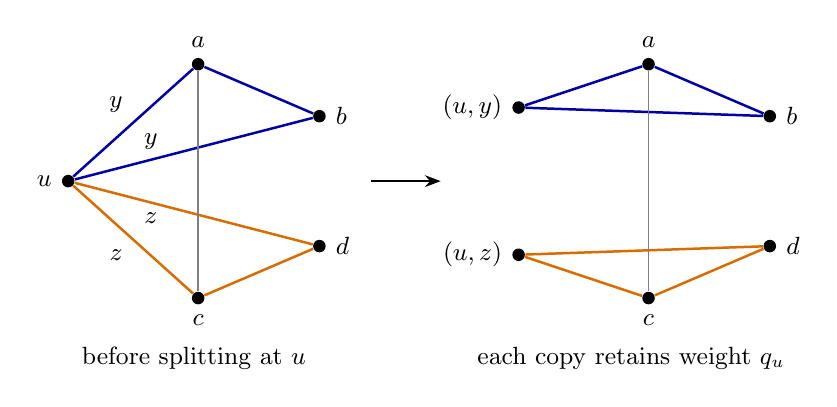
\begin{tikzpicture}[x=1.1cm,y=1.1cm,
 vertex/.style={circle,fill=black,inner sep=1.6pt},
 blueedge/.style={draw=blue!65!black,line width=0.9pt},
 orangeedge/.style={draw=orange!85!black,line width=0.9pt},
 every node/.style={font=\small}]
 \node[vertex,label=left:$u$] (u) at (0,0) {};
 \node[vertex,label=above:$a$] (a) at (1.5,1.35) {};
 \node[vertex,label=right:$b$] (b) at (2.9,0.75) {};
 \node[vertex,label=below:$c$] (c) at (1.5,-1.35) {};
 \node[vertex,label=right:$d$] (d) at (2.9,-0.75) {};
 \draw[blueedge] (u)--node[above left]{$y$}(a)--(b);
 \draw[blueedge] (u)--node[pos=.32,above]{$y$}(b);
 \draw[orangeedge] (u)--node[below left]{$z$}(c)--(d);
 \draw[orangeedge] (u)--node[pos=.32,below]{$z$}(d);
 \draw[gray,line width=0.6pt] (a)--(c);
 \node at (1.45,-2.05) {before splitting at $u$};
 \draw[-{Stealth[length=2mm]},thick] (3.5,0)--(4.3,0);
 \node[vertex,label=left:{$(u,y)$}] (uy) at (5.2,0.85) {};
 \node[vertex,label=left:{$(u,z)$}] (uz) at (5.2,-0.85) {};
 \node[vertex,label=above:$a$] (aa) at (6.7,1.35) {};
 \node[vertex,label=right:$b$] (bb) at (8.1,0.75) {};
 \node[vertex,label=below:$c$] (cc) at (6.7,-1.35) {};
 \node[vertex,label=right:$d$] (dd) at (8.1,-0.75) {};
 \draw[blueedge] (uy)--(aa)--(bb)--(uy);
 \draw[orangeedge] (uz)--(cc)--(dd)--(uz);
 \draw[gray,line width=0.6pt] (aa)--(cc);
 \node at (6.5,-2.05) {each copy retains weight $q_u$};
\end{tikzpicture}
\caption{A local view of the splitting construction. All displayed
incidences are assumed to qualify, and labels at vertices other than $u$
are suppressed. These are auxiliary incidence labels, not colors in the
correspondence assignment. The incidences $ua,ub$ have label $y$, while $uc,ud$ have
label $z\ne y$. The triangles $uab$ and $ucd$ remain triangles after
splitting at $u$; $uac$ does not. Each old edge is used once, and each
copy of $u$ keeps its original weight. The coupling makes unequal labels
at a triangle corner rare in weighted average.}
\label{fig:vertex-splitting}
\end{figure}


An old triangle survives with its original mass if all six incidences
qualify and the two labels agree at each of its three corners.  In the
ordered triangle law, each incidence has marginal $\mu$, and each
corner has the law used in \eqref{eq:corner-row-agreement}.  A union
bound, followed by averaging with the triangle weights, shows that the
expected fraction of triangle mass lost is at most
\[
 O_r\!\left(\frac{\log\ell}{\sqrt\ell}
              +\sqrt{\frac{\log\ell}{\ell}}\right)
       =O_r\!\left(\frac{\log\ell}{\sqrt\ell}\right).
\]
Choose a realization retaining at least the expected lower bound.  The
projection to $F$ is a homomorphism injective on directed edges, and
composing it with the old map to $H_b$ preserves that property.  All
vertex weights and inherited data remain unchanged.  This proves
\eqref{eq:split-retention} and the lemma.
\end{proof}

\subsection{Iteration and completion of the adjustment lemma}
\label{subsec:triangle-iteration}

\begin{proof}[Proof of Proposition~\ref{prop:triangle-bound}]
Apply the deletions of Subsection~\ref{subsec:triangle-preparation} to
all levels, then Lemma~\ref{lem:triangle-splitting} to each nonempty
level graph.  Empty level graphs need no construction.  The resulting
graphs have neighborhood weights at most $e^{\sqrt\ell}$ and still
have homomorphisms into their original $H_b$ injective on directed
edges.  Combining the additive losses from deletion with
\eqref{eq:split-retention} gives
\begin{equation}
 T_{\mathrm{new}}\ge
 \left(1-C_2\frac{\log\ell}{\sqrt\ell}\right)T
       -C_3\frac{\log\ell}{\ell}M_x,
 \label{eq:triangle-iteration}
\end{equation}
where the constants depend only on $r$.  If the coefficient of $T$ is
negative, the inequality follows simply from $T_{\mathrm{new}}\ge0$.

Choose a sufficiently large constant $X\ge32$, depending only on $r$.
Starting at $\ell_0$, perform the reduction while $\ell>X$, replacing
$\ell$ by $\sqrt\ell$ each time.  Both losses in
\eqref{eq:triangle-iteration} are summable uniformly in the initial
value $\ell_0$.  To verify this explicitly, let
$p(s)=(\log s)/\sqrt s$.  This function is decreasing for sufficiently
large $s$, and
\[
 \frac{p(s^2)}{p(s)}=\frac2{\sqrt s}.
\]
In reverse order, the parameters at which reductions are performed
start above $X$ and are successively squared.  Increasing $X$ therefore
makes the sum of $C_2p(\ell)$ at most $1/2$.  The sum of
$C_3(\log\ell)/\ell$ is bounded by a constant depending only on $r$.
Iterating \eqref{eq:triangle-iteration}, and using
$\prod_j(1-a_j)\ge1-\sum_ja_j$ for these nonnegative losses, gives
\begin{equation}
 T_{\mathrm{final}}\ge\frac12T_0-O_r(M_x).
 \label{eq:iterated-triangle-retention}
\end{equation}

At the final stage every neighborhood has weight at most $e^X$.
Every triangle still has a middle vertex.  At a middle vertex $a$,
the incident triangle mass, including the factor $b$, is at most
$bq_aq(N(a))^2/2$.  Hence \eqref{eq:middle-edge-charge} gives
\[
 T_{\mathrm{final}}
 \le\frac{e^X}{2}
      \sum_b b\sum_{\substack{a\in V(F_b)\\a\text{ middle}}}
                     q_aq(N(a))
 \le e^XM_x.
\]
This estimate also applies if $\ell_0\le X$ and no reduction is needed.
Together with \eqref{eq:iterated-triangle-retention}, it proves
$T_0=O_r(M_x)$.
\end{proof}

\begin{proof}[Completion of the proof of Lemma~\ref{lem:adjustment}]
Proposition~\ref{prop:triangle-bound} bounds the contribution from
triangles all of whose vertices are good by $O_r(M_x)$.  The contribution
from triangles meeting a bad vertex is, by \eqref{eq:bad-triangles}, at
most $O(\Lambda^2)\sum_iw_iy_i$.  Taking $B=B(r)$ sufficiently large
and then increasing the lower threshold on $\Lambda$ gives
\[
 \sum_i x_it_i\le B\sum_i x_id_i+\Lambda^4\sum_iw_iy_i,
\]
which is the dual inequality \eqref{eq:dual-target}.  The separation
argument in Section~\ref{sec:adjustment} now supplies the finite family
of operations and rates in \eqref{eq:adjustment}.  The constants are
chosen in order: first the multiplier bound $A$ and the local estimate
constant $C_1$, then the reduction constants and $X$, and finally $B$
and the threshold on $\Lambda$.  Every choice depends only on $r$, as
required.
\end{proof}

\section{Coloring rounds with dependent entry weights}\label{sec:rounds}

We now use Lemma~\ref{lem:adjustment} to extend a partial correspondence
coloring while controlling the weights of the entries that remain
available.  Entropy and edge energy, together with compensated weight
changes, are features of Johansson's coloring method; see
\cite[Sections~2 and~6--8]{BansalGuptaGuruganesh2018}.  Here the adjustment
operations act on the graph of list entries.  Entries in a single list need not evolve
independently; the bound on the number of entries from each part in an
operation will supply the concentration needed for a simultaneous update.

Fix $r\ge4$ and let $B=B(r)$ be the constant in
Lemma~\ref{lem:adjustment}.  Choose
\begin{equation}\label{eq:round-constants}
 K=16(B+2),\qquad \gamma=0.003,\qquad C=\frac{100K}{\gamma},\qquad
 k=\left\lceil\frac{C\Delta}{\log\Delta}\right\rceil.
\end{equation}
We prove Theorem~\ref{thm:main} with $C_r=C$.  Restrict each list to
exactly $k$ entries, restricting the matchings accordingly, and continue
to write $L(v)$ for the resulting lists.  For sufficiently large
$\Delta$ we have $k\le\Delta$.  Throughout the coloring process, $\Delta$
denotes the maximum degree of the original graph.  Set
\begin{equation}\label{eq:round-parameters}
 w_* = \frac Kk,\qquad \Lambda=20\log\Delta,\qquad
 \tau=\Delta^{-0.10},\qquad \xi=\Delta^{-0.14},\qquad
 \zeta=\Delta^{-0.15}.
\end{equation}
The parameter $\tau$ sets the activation and adjustment rates, $\xi$ is
the permitted error per round, and $\zeta$ is a smaller tolerance used
in the concentration estimates.
All asymptotic estimates below are uniform over the graphs, lists,
matchings, and states satisfying the stated assumptions, with $r$ fixed.
In particular, a factor $\Delta^{o(1)}$ in an upper bound is at most
$\Delta^\varepsilon$ for every fixed $\varepsilon>0$ once $\Delta$ is
sufficiently large in terms of $r$ and $\varepsilon$.  The parameters
$U,P_0$ in Lemma~\ref{lem:adjustment} are $\Delta^{o(1)}$, and
$R_0=O(\log\log\Delta)$, at the value of $\Lambda$ in
\eqref{eq:round-parameters}.

Consider a proper partial correspondence coloring, and let $G'$ be the
subgraph induced by its uncolored vertices.  An entry at an uncolored
vertex is \emph{available} if it conflicts with none of the colors already
chosen at neighboring vertices.  Give each entry $i\in L(v)$, for
$v\in V(G')$, a nonnegative weight $w_i$, requiring every positive-weight
entry to be available.  Let $H$ be the graph on the positive-weight
entries whose edges are the forbidden pairs in the restricted matchings.
Its parts are the sets $L(v)\cap V(H)$.  The map sending an entry to its
host vertex is a graph homomorphism $H\to G'$.  A clique in $H$ has
distinct hosts, so $H$ is $K_r$-free.  The matching condition also implies
that each entry has at most one neighbor in any part.  These are precisely
the structural assumptions of Lemma~\ref{lem:adjustment}.

Use $s_i,d_i,t_i$ for the neighborhood, incident-edge, and triangle
weights in that lemma, calculated in $H$.  We maintain
\begin{equation}\label{eq:weight-bounds}
 \Delta^{-3}\le w_i\le\Delta^{-0.99},\qquad s_i\le\Lambda
 \quad (i\in V(H)).
\end{equation}
For $v\in V(G')$ and $vu\in E(G')$, define
\begin{equation}\label{eq:vertex-potentials}
 \begin{aligned}
 W_v&=\sum_{i\in L(v)}w_i,\\
 D_{vu}&=\sum_{\substack{i\in L(v),\ l\in L(u)\\il\in E(H)}}w_iw_l,
 &D_v&=\sum_{u\in N_{G'}(v)}D_{vu},\\
 F_v&=\sum_{i\in L(v)}w_*f(w_i/w_*)
       +\gamma\log\Delta\,(K-W_v)+D_v.
 \end{aligned}
\end{equation}
The entropy sum includes zero-weight entries, using $f(0)=1$.
Both that sum and $D_v$ are nonnegative, and
$D_v=\sum_{i\in L(v)\cap V(H)}d_i\le\Lambda W_v$.
Thus an upper bound on $F_v$ prevents the total weight $W_v$ from
becoming too small, while coloring neighbors decreases its edge term.

Initially, color no vertices and give every entry weight $w_*$.  Since
$w_*=\Theta(\log\Delta/\Delta)$ and
$s_i\le\Delta w_*\le(K/C)\log\Delta$, the bounds
\eqref{eq:weight-bounds} hold.  Moreover,
\begin{equation}\label{eq:initial-state}
 W_v=K,\qquad F_v=D_v\le \frac{K^2\Delta}{k}
                         \le\frac{K^2}{C}\log\Delta.
\end{equation}
The following proposition is the step we shall iterate.

\begin{proposition}[One coloring round]\label{prop:one-round}
For all sufficiently large $\Delta$ depending only on $r$, suppose that
a proper partial correspondence coloring and entry weights satisfy
availability, \eqref{eq:weight-bounds}, and
\begin{equation}\label{eq:mass-window}
 K/2\le W_v\le2K\qquad(v\in V(G')).
\end{equation}
There is an extension of the partial coloring and a choice of weights
on the remaining entries that preserve availability and
\eqref{eq:weight-bounds}, and satisfy
\begin{equation}\label{eq:round-conclusions}
 W_v^{\mathrm{new}}\le W_v+\xi,\qquad
 F_v^{\mathrm{new}}\le F_v+\xi,\qquad
 \frac{\deg_{\mathrm{new}}(v)}{\Delta}
 \le(1-\tau)\frac{\deg_{G'}(v)}{\Delta}+\xi
\end{equation}
for every vertex $v$ that remains uncolored.
\end{proposition}

\subsection{The random update and its expectation}

Assume the hypotheses of Proposition~\ref{prop:one-round}; the case
$V(G')=\varnothing$ is immediate.  Fix the operations and rates $a_j$
given by Lemma~\ref{lem:adjustment} on $H$, with listed supports $J_j$.
We use two families of mutually independent Bernoulli flags.  For each
entry $z\in V(H)$ an \emph{activation flag} is set with probability
$\tau w_z$; it touches every neighbor of $z$ in $H$, with designated
multiplier zero there.  For each operation $j$ its flag is set with
probability $\tau a_j$ and touches $J_j$.  A multiplier operation has
its prescribed multipliers $m_i^{(j)}$ on $J_j$, and a drop has designated
multiplier zero on its singleton support.  The probabilities are valid
for large $\Delta$: the nonempty support and rate bound of
Lemma~\ref{lem:adjustment} give $a_j\le\Lambda^4$.

For each $i\in V(H)$ put $\bar w_i=w_iY_i$.  If exactly one set flag
touches $i$, let $Y_i$ be its designated multiplier; if at least two set
flags touch $i$, let $Y_i=0$.  If no set flag touches $i$, put
\begin{equation}\label{eq:no-flag-multiplier}
 Y_i=1+\tau\left(s_i+\sum_{j\in\mathcal M}a_j(1-m_i^{(j)})\right),
\end{equation}
where $\mathcal M$ indexes the multiplier operations and their
multipliers are extended by $1$ off the listed supports.  Zero-weight
entries stay at zero.  The coefficient of $\tau$ in
\eqref{eq:no-flag-multiplier} has absolute value at most
$\Lambda+\Lambda^4(1+U)$.  The no-flag multiplier is therefore positive
and is $1+O(\tau\Delta^{o(1)})$.

An entry \emph{activates} when its activation flag is set.  An activating
entry is \emph{successful} if none of its neighbors in $H$ activates.
At every host with a successful entry, choose one such entry as its color,
using any fixed order on that list to break ties.  Successful entries
cannot be adjacent in $H$, and they were available before the round,
so this extends the proper partial coloring.  Every entry conflicting
with a newly chosen color is touched by its activation flag and hence
has provisional weight zero, whether or not other flags also touch it.
Consequently, after newly colored vertices are removed, all remaining
positive provisional weights are available.
The set of hosts receiving a color depends only on activation flags,
independently of the choices among successful entries.

Until that removal, a bar on any quantity in
\eqref{eq:vertex-potentials} means that it is calculated with the
provisional weights on the entire start-of-round graph $G'$.  We may
continue to use $E(H)$ in these sums because zero weights remain zero.
The compensation in \eqref{eq:no-flag-multiplier} cancels the
first-order mean loss from activations and multiplier operations.
The following estimate shows how the adjustment lemma controls the
remaining cost in the potential.

\begin{lemma}[Expected changes]\label{lem:round-expectation}
For the random update just defined,
\begin{equation}\label{eq:round-expectations}
 \begin{aligned}
 \EE\bar W_v&\le W_v+o(\xi),\\
 \EE\bar F_v&\le F_v+\tau(B+1)D_v+o(\xi),\\
 \EE\bar D_{vu}&\ge\tfrac12D_{vu}\qquad(vu\in E(G')).
 \end{aligned}
\end{equation}
\end{lemma}

\begin{proof}
Let $a_i^-$ be the sum of the rates of drops at $i$.  Expanding according
to the set flags touching one or two entries gives the following
identities, with $il\in E(H)$ in the last line:
\begin{equation}\label{eq:multiplier-moments}
 \begin{aligned}
 \EE(Y_i-1)
   &=-\tau a_i^-+O(\tau^2\Delta^{o(1)}),\\
 \EE f(Y_i)
   &=\tau\left(s_i+a_i^-+
           \sum_{j\in\mathcal M}a_jf(m_i^{(j)})\right)
       +O(\tau^2\Delta^{o(1)}),\\
 \EE[(Y_i-1)(Y_l-1)]
   &=\tau\sum_{z\in N_H(i)\cap N_H(l)}w_z\\
   &\quad+\tau\sum_{j\in\mathcal M}
          a_j(m_i^{(j)}-1)(m_l^{(j)}-1)
       +O(\tau^2\Delta^{o(1)}).
 \end{aligned}
\end{equation}
Here is a justification of the errors and the first-order terms.
The sum of the probabilities of flags touching either of two fixed
entries is at most $2\tau(\Lambda+\Lambda^4)$.  Independence bounds
both the probability of two or more such flags and the total error in
replacing the exact single-flag probabilities by their marginal probabilities by
$O(\tau^2\Delta^{o(1)})$.  All multipliers and their $f$-values are
$\Delta^{o(1)}$, so these errors remain of the stated order.
For the first line, the single flags contribute
$-s_i-a_i^-+\sum_{j\in\mathcal M}a_j(m_i^{(j)}-1)$ to the coefficient
of $\tau$; \eqref{eq:no-flag-multiplier} cancels all but $-a_i^-$.
For the second line, use $f(0)=1$ and $f(1+h)=O(h^2)$ at the no-flag
value.  For the third line, only flags touching both entries contribute
to first order.  These are common-neighbor activations and shared
multiplier flags.  A singleton drop cannot touch both endpoints, and
a flag touching only one endpoint has an additional factor
$O(\tau\Delta^{o(1)})$ from the other endpoint.

For every $i\in V(H)$, including when $Y_i=0$, the entropy identity is
\begin{equation}\label{eq:entropy-change}
 w_*\bigl[f(w_iY_i/w_*)-f(w_i/w_*)\bigr]
   =w_i\log(w_i/w_*)(Y_i-1)+w_if(Y_i).
\end{equation}
Allocate the change in $F_v$ to its positive-weight entries.  The
contribution of $i\in L(v)\cap V(H)$ is
\begin{equation}\label{eq:entry-potential-change}
 w_i\bigl[(\log(w_i/w_*)-\gamma\log\Delta)(Y_i-1)+f(Y_i)\bigr]
 +\sum_{l\in N_H(i)}w_iw_l(Y_iY_l-1).
\end{equation}
Its expectation is at most
\begin{equation}\label{eq:entry-expected-change}
 \tau\left(d_i+t_i+\sum_j a_jg_i^{(j)}\right)
 +O\bigl((w_i+d_i)\tau^2\Delta^{o(1)}\bigr).
\end{equation}
Indeed, \eqref{eq:multiplier-moments} gives the activation terms $d_i$
from entropy and $t_i$ from edge correlations.  For a multiplier
operation, the compensated linear terms cancel, leaving exactly
$w_if(m_i^{(j)})$ and the quadratic edge terms that define $g_i^{(j)}$.
A drop at $i$ contributes
$w_i(1-\log(w_i/w_*)+\gamma\log\Delta)\le\Lambda w_i$ to the
non-edge part and $-d_i$ to the edge part.  A drop at a neighbor $l$
contributes $-w_iw_l$.  These are bounded by the drop vector in
Lemma~\ref{lem:adjustment}.  Finally,
$|\log(w_i/w_*)|=O(\log\Delta)$ by \eqref{eq:weight-bounds}; absorbing
these logarithms gives the error in \eqref{eq:entry-expected-change}.

Sum \eqref{eq:entry-expected-change} over $L(v)\cap V(H)$ and use
$t_i+\sum_j a_jg_i^{(j)}\le Bd_i$.  Since
$D_v\le\Lambda W_v$ and $W_v\le2K$, the total error is
$O((W_v+D_v)\tau^2\Delta^{o(1)})=o(\xi)$.  This proves the potential
estimate.  The first line of \eqref{eq:multiplier-moments} proves the
mass estimate.  For each edge $il$ in the sum defining $D_{vu}$, the
probability that neither endpoint is touched by a set flag is
$1-O(\tau\Delta^{o(1)})$; on this event,
$Y_iY_l=1+O(\tau\Delta^{o(1)})$.  Nonnegativity on the other events
therefore gives $\EE(w_iw_lY_iY_l)\ge w_iw_l/2$ for large $\Delta$.
Summing proves the last assertion.
\end{proof}

\subsection{Concentration with bounded input participation}

We next make the expectation bounds simultaneous at all vertices.
The relevant concentration principle is a bounded-variable form of
the generalized H\"older inequality of Finner~\cite{Finner} and the
read-$k$ concentration method of Gavinsky, Lovett, Saks, and
Srinivasan~\cite{GavinskyReadK}.  We give the short proof, including
the exponential-moment estimate of Hoeffding~\cite{Hoeffding1963}.

\begin{lemma}[Bounded input participation]\label{lem:read-concentration}
Let $X_1,\ldots,X_m$ be bounded real functions of finitely many
independent inputs.  Suppose that $X_j$ has range of length at most
$b_j$, and that each input is used by at most $p$ of the functions,
where $p\ge1$ is real.  If $\sum_jb_j^2>0$, then for every $a>0$,
\begin{equation}\label{eq:input-concentration}
 \PP\left(\sum_j(X_j-\EE X_j)\ge a\right),\quad
 \PP\left(\sum_j(X_j-\EE X_j)\le-a\right)
 \ \le\ \exp\left(-\frac{2a^2}{p\sum_jb_j^2}\right).
\end{equation}
If $\sum_jb_j^2=0$, both probabilities are zero.
\end{lemma}

\begin{proof}
For nonnegative bounded functions $Z_j$ with the same dependence
sets, we first prove
\begin{equation}\label{eq:input-holder}
 \EE\prod_j Z_j\le\prod_j(\EE Z_j^p)^{1/p}.
\end{equation}
Induct on the number of independent inputs.  Condition on all inputs
except the last, and let $I$ index the functions using that last input.
H\"older's inequality with exponent $p$ for the $|I|\le p$ factors,
and with a constant factor $1$ of reciprocal exponent $1-|I|/p$ when
$|I|<p$, bounds this conditional integral
by $\prod_j\widetilde Z_j$, where
$\widetilde Z_j=(\EE_{\mathrm{last}}Z_j^p)^{1/p}$ for $j\in I$ and
$\widetilde Z_j=Z_j$ otherwise.  Each $\widetilde Z_j$ uses only the
remaining inputs of $Z_j$, so the participation bound still holds.
The induction hypothesis applies and gives
$\EE\prod_j\widetilde Z_j\le
\prod_j(\EE\widetilde Z_j^p)^{1/p}
=\prod_j(\EE Z_j^p)^{1/p}$, proving \eqref{eq:input-holder}.

If a random variable $X$ has range of length $b$, then
\begin{equation}\label{eq:hoeffding-moment}
 \log\EE e^{s(X-\EE X)}\le\frac{s^2b^2}{8}\qquad(s\in\mathbb R).
\end{equation}
To see this, the second derivative of the logarithm on the left is
the variance under the exponentially tilted law.  Any law supported
on an interval of length $b$ has variance at most $b^2/4$, by measuring
squared distance from the midpoint.  The logarithm and its first
derivative vanish at zero, which proves \eqref{eq:hoeffding-moment}.
Apply \eqref{eq:input-holder} to
$Z_j=e^{s(X_j-\EE X_j)}$ and then \eqref{eq:hoeffding-moment} with
parameter $ps$.  The resulting moment bound is
$\exp(ps^2\sum_jb_j^2/8)$.  Exponential Markov with
$s=4a/(p\sum_jb_j^2)$ proves the upper tail; replacing $X_j$ by
$-X_j$ proves the lower tail.
\end{proof}

Apply Lemma~\ref{lem:read-concentration} first to $\bar W_v$ and to
the non-edge part $\bar F_v-\bar D_v$.  Apart from an additive constant,
each is a sum of at most $k\le\Delta$ functions, one for each entry of
$L(v)$, of range length at most $\Delta^{-0.99+o(1)}$.  This follows
from \eqref{eq:weight-bounds}, \eqref{eq:no-flag-multiplier}, and
$U=\Delta^{o(1)}$; the logarithmic factors in the entropy term are
absorbed in $\Delta^{o(1)}$.  This also covers arbitrarily small
positive provisional weights: with $0\log0=0$,
$\sup_{0\le z\le b}|z\log z|=b\log(1/b)$ for $0<b<e^{-1}$.
A multiplier flag occurs in at most
$P_0$ of these functions, by its support bound in a single part.
A drop flag occurs in at most one, and an activation flag occurs in
at most one because its activating entry has at most one neighbor
in $L(v)$.  Thus $p=P_0$ is valid.  In particular, each requirement
\begin{equation}\label{eq:vertex-concentration}
 \bar W_v\le\EE\bar W_v+\zeta,\qquad
 \bar F_v-\bar D_v\le\EE(\bar F_v-\bar D_v)+\zeta
\end{equation}
fails with probability at most $\exp(-\Delta^{0.5})$ for large $\Delta$:
the exponent in \eqref{eq:input-concentration} is at least
$\Delta^{0.68-o(1)}$.

For an edge $vu\in E(G')$, the matching sum $\bar D_{vu}$ has at
most $k$ terms, each of range length at most
$\Delta^{-1.98+o(1)}$.  Every entry at either endpoint occurs in at
most one term, so each flag occurs in at most $2P_0$ terms.  Applying
Lemma~\ref{lem:read-concentration} with $p=2P_0$ shows that
\begin{equation}\label{eq:matching-concentration}
 |\bar D_{vu}-\EE\bar D_{vu}|\le\Delta^{-1.25}
\end{equation}
fails with probability at most $2\exp(-\Delta^{0.4})$.  Here the
exponent is at least $\Delta^{0.46-o(1)}$.  This separation into
non-edge terms and individual matching sums is what permits the
participation bound to apply; no independence among entries of a
list is assumed.

For ordinary list coloring, operations can instead be chosen separately
in each graph induced by one common color label.  Sampling their flags
independently makes contributions of distinct colors independent, so
the corresponding concentration bound has $p=1$.  Arbitrary edge
matchings provide no such common labels; the per-part support bound
replaces that independence here.

\subsection{Activations that produce colors}

The expectation estimate allows a potential increase of order
$\tau D_v$.  To offset it, we must show that enough neighbors receive
colors, with their contributions measured both by $D_{vu}$ and by
$1/\Delta$.  Fix $v\in V(G')$, and take one of the coefficient families
\begin{equation}\label{eq:neighbor-coefficients}
 b_u=D_{vu}\quad(u\in N_{G'}(v)),\qquad\text{or}\qquad
 b_u=1/\Delta\quad(u\in N_{G'}(v)).
\end{equation}
In either case $0\le b_u\le2K\Delta^{-0.99}$: for the first family,
the matching property gives $D_{vu}\le\Delta^{-0.99}W_v$.
Let $A_u$ indicate that some entry at $u$ activates.  These indicators
are independent over the hosts $u$, and
\begin{equation}\label{eq:host-activation-probability}
 \PP(A_u=1)\ge1-e^{-\tau W_u}\ge\tau K/4
\end{equation}
for large $\Delta$, since $K/2\le W_u\le2K$.
Lemma~\ref{lem:read-concentration} with $p=1$ and
$\sum_ub_u^2\le4K^2\Delta^{-0.98}$ gives
\begin{equation}\label{eq:activated-neighbor-mass}
 \sum_{u\in N_{G'}(v)}b_uA_u
 \ge\frac{\tau K}{4}\sum_{u\in N_{G'}(v)}b_u-\zeta
\end{equation}
except with probability at most $\exp(-\Delta^{0.5})$.
The next lemma bounds the loss caused by conflicting activations.

\begin{lemma}[Collision bound]\label{lem:activation-collisions}
Let $\mathcal E_v$ be the set of edges of $H$ with an endpoint hosted
at a neighbor of $v$ in $G'$, and let $X_v$ count the edges of
$\mathcal E_v$ whose two endpoints activate.  Then
\begin{equation}\label{eq:collision-tail}
 \PP\bigl(4K\Delta^{-0.99}X_v>\zeta\bigr)
 \le O(\Delta^3)e^{e-1-\Delta^{0.01}}+e^{-\Delta^{0.8}}.
\end{equation}
For either coefficient family in \eqref{eq:neighbor-coefficients},
the sum of $b_u$ over hosts $u$ counted by $A_u$ that receive no
color is at most $4K\Delta^{-0.99}X_v$.
\end{lemma}

\begin{proof}
A host with an activating entry but no successful entry contains an
endpoint of an edge counted by $X_v$.  Each such edge has at most
two hosts and each coefficient is at most $2K\Delta^{-0.99}$, proving
the final assertion.  Moreover,
\begin{equation}\label{eq:collision-expectation}
 \mu_v:=\EE X_v
 \le\tau^2\sum_{u\in N_{G'}(v)}
               \sum_{i\in L(u)\cap V(H)}w_is_i
 \le2K\Delta\tau^2\Lambda=\Delta^{0.80+o(1)}.
\end{equation}

For a possible endpoint $i$ of an edge in $\mathcal E_v$, the number
of its activating neighbors is a sum of independent indicators of
total mean $\tau s_i\le\tau\Lambda\le1$.  Its exponential moment at
parameter $1$ is at most $\exp(e-1)$, so it exceeds
$\Delta^{0.01}$ with probability at most
$\exp(e-1-\Delta^{0.01})$.  All possible endpoints are hosted within
distance two of $v$ in $G'$, and there are at most $k\le\Delta$ entries
at each host.  A union bound over $O(\Delta^3)$ endpoints shows that,
apart from the first error term in \eqref{eq:collision-tail}, the
graph formed by the edges counted by $X_v$ has maximum degree at
most $\Delta^{0.01}$.

If $4K\Delta^{-0.99}X_v>\zeta$, then
$X_v>\Delta^{0.84}/(4K)$.  In a graph of maximum degree at most
$\Delta^{0.01}$, greedy selection of disjoint edges produces a matching
of size at least $X_v/(2\Delta^{0.01})$.  For large $\Delta$ this is
at least $m=\lceil\Delta^{0.82}\rceil$.  For $e=il\in\mathcal E_v$
write $q_e=\tau^2w_iw_l$.  The events that both endpoints activate
are independent along any matching, because its edges have disjoint
endpoints and the activation flags are independent.  Consequently,
\begin{equation}\label{eq:collision-matching-tail}
 \begin{aligned}
 \PP\left(\begin{gathered}
     \text{some size-$m$ matching in $\mathcal E_v$}\\
     \text{has all endpoints activating}
   \end{gathered}\right)
 &\le\sum_{\substack{M\subseteq\mathcal E_v\\M\text{ matching},\ |M|=m}}
                      \prod_{e\in M}q_e\\
 &\le\frac{(\sum_{e\in\mathcal E_v}q_e)^m}{m!}
   =\frac{\mu_v^m}{m!}
   \le\left(\frac{e\mu_v}{m}\right)^m
   \le e^{-\Delta^{0.8}}.
 \end{aligned}
\end{equation}
The second inequality follows by expanding the power: each matching
appears $m!$ times, and all other terms are nonnegative.  The final
inequality uses \eqref{eq:collision-expectation} and
$m=\Delta^{0.82+o(1)}$; it is immediate if $\mu_v=0$.
Combining the two exceptional events proves the lemma.
\end{proof}

Together, \eqref{eq:activated-neighbor-mass} and
Lemma~\ref{lem:activation-collisions} imply that, for either choice
in \eqref{eq:neighbor-coefficients}, we may require
\begin{equation}\label{eq:colored-neighbor-mass}
 \sum_{\substack{u\in N_{G'}(v)\\u\text{ receives a color}}}b_u
 \ge\frac{\tau K}{4}\sum_{u\in N_{G'}(v)}b_u-2\zeta.
\end{equation}
Let $E_v$ be the event that \eqref{eq:vertex-concentration},
\eqref{eq:matching-concentration} for an edge incident with $v$, or
\eqref{eq:colored-neighbor-mass} for one of the two coefficient
families fails.  A union bound gives, for all sufficiently large
$\Delta$,
\begin{equation}\label{eq:round-failure-probability}
 \PP(E_v)\le\exp(-\Delta^{0.005}).
\end{equation}

\subsection{Simultaneous bounds and restoration of the weight conditions}

We use the Lov\'asz local lemma~\cite{ErdosLovasz1975} to avoid every
$E_v$.  Assign each multiplier flag to the host of a chosen center of
a radius-$R_0$ ball in $H$ containing its listed support.  Assign
activation and drop flags to the hosts of the activating and dropped
entries, respectively.  Every input determining $E_v$ is assigned
within distance $R_0+3$ of $v$ in $G'$.  Indeed, the host projection
does not increase distances; the provisional weights on an incident
matching use flags touching entries at its two hosts; and whether
a neighbor of $v$ receives a color is determined by activation flags
at distance at most two from $v$.  Events at distance greater than
$2(R_0+3)$ therefore involve disjoint sets of independent inputs.
A bound for the maximum degree of a dependency graph is
\begin{equation}\label{eq:round-dependency-degree}
 d=(\Delta+1)^{2R_0+10}
   \le\exp\bigl(O(\log\Delta\log\log\Delta)\bigr).
\end{equation}

For completeness, the symmetric local lemma says that finitely many
events of probability at most $q$, with a dependency graph of maximum
degree at most $d\ge1$, can all be avoided if
$q\le1/(e(d+1))$.  Put $x=1/(d+1)$, so
$q\le x(1-x)^d$.  Induction on the number of conditioned events shows
that any event, conditioned on the avoidance of any set of the others,
has probability at most $x$.  To make the induction step, split the
conditioning set into nonneighbors and at most $d$ neighbors of the
event.  Independence bounds the numerator after conditioning on the
nonneighbors by $q$, and the induction hypothesis bounds the
probability of avoiding the neighbors, under that conditioning, below
by $(1-x)^d$.  The same induction ensures that all conditioning
probabilities are positive.  Multiplying these positive conditional
avoidance probabilities proves joint avoidance.  By
\eqref{eq:round-failure-probability} and
\eqref{eq:round-dependency-degree}, its hypothesis holds here for
large $\Delta$.

\begin{proof}[Proof of Proposition~\ref{prop:one-round}]
Fix a trial avoiding all $E_v$.  Lemma~\ref{lem:round-expectation},
\eqref{eq:vertex-concentration}, and
\eqref{eq:matching-concentration} summed over the edges incident
with $v$ give
\begin{equation}\label{eq:provisional-bounds}
 \bar W_v\le W_v+o(\xi),\qquad
 \bar F_v\le F_v+\tau(B+1)D_v+o(\xi),
\end{equation}
because $\zeta+\Delta\Delta^{-1.25}=o(\xi)$.
Remove the vertices colored in this trial.  At a remaining vertex
$v$, only the edge part of its potential changes.  Each removed
neighbor $u$ contributes
$\bar D_{vu}\ge D_{vu}/2-\Delta^{-1.25}$ by
\eqref{eq:round-expectations} and
\eqref{eq:matching-concentration}.  Using
\eqref{eq:colored-neighbor-mass} with $b_u=D_{vu}$, the total
decrease is at least
\begin{equation}\label{eq:potential-removal-gain}
 \sum_{\substack{u\in N_{G'}(v)\\u\text{ receives a color}}}\bar D_{vu}
 \ge\frac{\tau K}{8}D_v-\zeta-\Delta^{-0.25}.
\end{equation}
Since $K/8>B+1$, the potential after removal is at most $F_v+o(\xi)$.
The same requirement with $b_u=1/\Delta$ gives the degree bound in
\eqref{eq:round-conclusions}, because $K/4\ge1$ and $2\zeta=o(\xi)$.
It remains to restore \eqref{eq:weight-bounds} without losing the
mass and potential estimates.

To \emph{trim} an entry means to set its weight to zero.  If its
current positive weight is $z$, the change in the non-edge part of
its host's potential is exactly
\begin{equation}\label{eq:trimming-cost}
 c(z):=z\bigl(1-\log(z/w_*)+\gamma\log\Delta\bigr).
\end{equation}
First trim all entries with $z>\Delta^{-0.99}$.  Their costs are
nonpositive for large $\Delta$, since
$\log(\Delta^{-0.99}/w_*)=0.01\log\Delta-O(\log\log\Delta)$ and
$\gamma<0.01$.  Next trim all positive entries with $z<\Delta^{-3}$.
The function $c(z)$ is increasing on this interval for large $\Delta$
and has limit zero at zero, so each cost is at most
$O(\Delta^{-3}\log\Delta)$.  There are at most $k\le\Delta$ entries
at a host, giving total cost $o(\xi)$ there.  Both trimming operations
can only decrease edge terms.

At the resulting weights, mark each positive entry $i$ with
$s_i>\Lambda$, and trim all marked entries simultaneously.  For a
marked entry of weight $z$, \eqref{eq:trimming-cost} is at most
$\Lambda z$ on the restored weight interval.  To account for the
edge loss without double counting, let $M$ be the marked entries and
fix a host $v$.  In the next identity, $H,w_i,s_i,D_v$ refer to the
remaining graph and weights immediately before this last trim, and
$D'_v$ is the edge term after it.  Then
\begin{equation}\label{eq:simultaneous-trimming-loss}
 D_v-D'_v
 =\sum_{i\in M\cap L(v)}w_is_i
  +\sum_{i\in (V(H)\setminus M)\cap L(v)}
       w_i\sum_{l\in M\cap N_H(i)}w_l
 \ge\sum_{i\in M\cap L(v)}w_is_i.
\end{equation}
Each deleted edge in $D_v$ has exactly one endpoint hosted at $v$, so
it occurs in precisely one of these two sums.  The first sum pays for
all non-edge costs at $v$, since $w_is_i>\Lambda w_i$ for marked
entries.  This remains true when both ends of an edge are trimmed.
This last trim does not
increase any $F_v$.  The unmarked entries had $s_i\le\Lambda$ before
the trim, and deleting weights only reduces their neighborhood
weights, so the remaining entries satisfy \eqref{eq:weight-bounds}.

All trims preserve availability and do not increase $W_v$.  Combining
their costs with \eqref{eq:provisional-bounds} and
\eqref{eq:potential-removal-gain} proves the mass and potential bounds
in \eqref{eq:round-conclusions} for sufficiently large $\Delta$.
\end{proof}

\section{Iteration and completion}\label{sec:completion}

We finish the proof of Theorem~\ref{thm:main} by iterating
Proposition~\ref{prop:one-round}.  The potential keeps a fixed positive
amount of weight at each remaining vertex, while the maximum remaining
degree decreases to a smaller order than the number of available
positive-weight entries.

\begin{proof}[Proof of Theorem~\ref{thm:main}]
Start from the empty partial coloring and the weights in
\eqref{eq:initial-state}, and set
\begin{equation}\label{eq:number-of-rounds}
 T_* = \left\lceil2\tau^{-1}\log\Delta\right\rceil.
\end{equation}
Perform $T_*$ rounds, stopping earlier if every vertex receives a
color.  We verify inductively that the mass assumption
\eqref{eq:mass-window} remains valid.  After $j\le T_*$ completed
rounds, every remaining vertex satisfies
\begin{equation}\label{eq:iteration-potentials}
 W_v\le K+j\xi,\qquad
 \gamma\log\Delta\,(K-W_v)\le F_v
 \le\frac{K^2}{C}\log\Delta+j\xi.
\end{equation}
The upper bounds follow from \eqref{eq:initial-state} and
\eqref{eq:round-conclusions}; the lower bound on $F_v$ follows from
the nonnegative entropy and edge terms in
\eqref{eq:vertex-potentials}.  Since
$T_*\xi=O(\Delta^{-0.04}\log\Delta)=o(1)$ and
$C=100K/\gamma$, these inequalities give
\begin{equation}\label{eq:iteration-mass-window}
 K-\frac K{100}-\frac{T_*\xi}{\gamma\log\Delta}
 \le W_v\le K+T_*\xi.
\end{equation}
For sufficiently large $\Delta$, both bounds lie inside $[K/2,2K]$.
Availability and \eqref{eq:weight-bounds} are preserved by the
proposition, so each successive round is justified.

If vertices remain after $T_*$ rounds, repeated use of the degree
inequality in \eqref{eq:round-conclusions} gives
\begin{equation}\label{eq:final-degree}
 \frac{\deg_{\mathrm{remaining}}(v)}{\Delta}
 \le(1-\tau)^{T_*}+\xi\sum_{j=0}^{T_*-1}(1-\tau)^j
 \le\Delta^{-2}+\frac{\xi}{\tau}
 =\Delta^{-2}+\Delta^{-0.04}.
\end{equation}
On the other hand, the mass lower bound and the upper bound on each
positive entry imply
\begin{equation}\label{eq:available-entry-count}
 \bigl|\{i\in L(v):w_i>0\}\bigr|
 \ge\frac K2\Delta^{0.99}.
\end{equation}
For large $\Delta$ this exceeds the remaining maximum degree, which
is at most $\Delta^{-1}+\Delta^{0.96}$ by \eqref{eq:final-degree}.
Color the remaining vertices in any order, choosing at each step a
positive-weight entry compatible with the colors already chosen.
Every such entry is available with respect to the partial coloring
from the rounds.  Each neighbor colored during this final procedure
forbids at most one entry, by the matching condition.  Inequality
\eqref{eq:available-entry-count} therefore guarantees a choice at
every step.

The resulting coloring chooses one entry from each restricted list
and avoids every forbidden pair, so it is also a coloring for the
original lists and matchings.  All lower thresholds on $\Delta$ in
the proof depend only on $r$.  Choosing a single
$\Delta_r\ge3$ above them, together with $C_r=C$ from
\eqref{eq:round-constants}, proves Theorem~\ref{thm:main}.
\end{proof}

\begin{thebibliography}{99}
\addcontentsline{toc}{section}{References}
\raggedright

\bibitem{AEKS1981}
M.~Ajtai, P.~Erd\H{o}s, J.~Koml\'os, and E.~Szemer\'edi,
On Tur\'an's theorem for sparse graphs,
\emph{Combinatorica} \textbf{1} (1981), no.~4, 313--317.
\url{https://doi.org/10.1007/BF02579451}.

\bibitem{AKS1999}
N.~Alon, M.~Krivelevich, and B.~Sudakov,
Coloring graphs with sparse neighborhoods,
\emph{J. Combin. Theory Ser. B} \textbf{77} (1999), no.~1, 73--82.
\url{https://doi.org/10.1006/jctb.1999.1910}.

\bibitem{AndersonBernshteynDhawan2023}
J.~Anderson, A.~Bernshteyn, and A.~Dhawan,
Colouring graphs with forbidden bipartite subgraphs,
\emph{Combin. Probab. Comput.} \textbf{32} (2023), no.~1, 45--67.
\url{https://doi.org/10.1017/S0963548322000104}.

\bibitem{AndersonBernshteynDhawan}
J.~Anderson, A.~Bernshteyn, and A.~Dhawan,
Coloring graphs with forbidden almost bipartite subgraphs,
\emph{Random Structures Algorithms} \textbf{66} (2025), no.~4, e70012.
\url{https://doi.org/10.1002/rsa.70012}.

\bibitem{AngelSpinka}
O.~Angel and Y.~Spinka,
\emph{Pairwise optimal coupling of multiple random variables},
arXiv:1903.00632 (2019), revised 2021.
\url{https://arxiv.org/abs/1903.00632}.

\bibitem{BansalGuptaGuruganesh2018}
N.~Bansal, A.~Gupta, and G.~Guruganesh,
On the Lov\'asz theta function for independent sets in sparse graphs,
\emph{SIAM J. Comput.} \textbf{47} (2018), no.~3, 1039--1055.
\url{https://doi.org/10.1137/15M1051002}.
Extended version: \url{https://arxiv.org/abs/1504.04767}.

\bibitem{BDKY2015}
I.~Benjamini, H.~Duminil-Copin, G.~Kozma, and A.~Yadin,
Disorder, entropy and harmonic functions,
\emph{Ann. Probab.} \textbf{43} (2015), no.~5, 2332--2373.
\url{https://doi.org/10.1214/14-AOP934}.

\bibitem{Bernshteyn2016}
A.~Bernshteyn,
The asymptotic behavior of the correspondence chromatic number,
\emph{Discrete Math.} \textbf{339} (2016), no.~11, 2680--2692.
\url{https://doi.org/10.1016/j.disc.2016.05.012}.

\bibitem{Bernshteyn2019}
A.~Bernshteyn,
The Johansson--Molloy theorem for DP-coloring,
\emph{Random Structures Algorithms} \textbf{54} (2019), no.~4, 653--664.
\url{https://doi.org/10.1002/rsa.20811}.

\bibitem{Bollobas1978}
B.~Bollob\'as,
Chromatic number, girth and maximal degree,
\emph{Discrete Math.} \textbf{24} (1978), no.~3, 311--314.
\url{https://doi.org/10.1016/0012-365X(78)90102-4}.

\bibitem{DKPSLocalOccupancy}
E.~Davies, R.~J.~Kang, F.~Pirot, and J.-S.~Sereni,
\emph{Graph structure via local occupancy},
arXiv:2003.14361 (2020).
\url{https://arxiv.org/abs/2003.14361}.

\bibitem{DhawanJanzerMethuku}
A.~Dhawan, O.~Janzer, and A.~Methuku,
\emph{Independent sets and colorings of $K_{t,t,t}$-free graphs},
arXiv:2511.17191 (2025), version~2.
\url{https://arxiv.org/abs/2511.17191}.

\bibitem{DvorakPostle}
Z.~Dvo\v{r}\'ak and L.~Postle,
Correspondence coloring and its application to list-coloring planar graphs
without cycles of lengths 4 to 8,
\emph{J. Combin. Theory Ser. B} \textbf{129} (2018), 38--54.
\url{https://doi.org/10.1016/j.jctb.2017.09.001}.

\bibitem{ErdosLovasz1975}
P.~Erd\H{o}s and L.~Lov\'asz,
Problems and results on $3$-chromatic hypergraphs and some related questions,
in \emph{Infinite and Finite Sets}, Vol.~II,
Colloq. Math. Soc. J\'anos Bolyai \textbf{10},
North-Holland, Amsterdam, 1975, pp.~609--627.
\url{https://www.renyi.hu/~p_erdos/1975-34.pdf}.

\bibitem{ErdosRubinTaylor1980}
P.~Erd\H{o}s, A.~L.~Rubin, and H.~Taylor,
Choosability in graphs,
in \emph{Proceedings of the West Coast Conference on Combinatorics,
Graph Theory and Computing} (Arcata, California, 1979),
Congr. Numer. \textbf{26}, Utilitas Math., Winnipeg, 1980, pp.~125--157.
\url{https://www.renyi.hu/~p_erdos/1980-07.pdf}.

\bibitem{Finner}
H.~Finner,
A generalization of H\"older's inequality and some probability inequalities,
\emph{Ann. Probab.} \textbf{20} (1992), no.~4, 1893--1901.
\url{https://doi.org/10.1214/aop/1176989534}.

\bibitem{GavinskyReadK}
D.~Gavinsky, S.~Lovett, M.~Saks, and S.~Srinivasan,
A tail bound for read-$k$ families of functions,
\emph{Random Structures Algorithms} \textbf{47} (2015), no.~1, 99--108.
\url{https://doi.org/10.1002/rsa.20532}.

\bibitem{Hoeffding1963}
W.~Hoeffding,
Probability inequalities for sums of bounded random variables,
\emph{J. Amer. Statist. Assoc.} \textbf{58} (1963), no.~301, 13--30.
\url{https://doi.org/10.1080/01621459.1963.10500830}.

\bibitem{Kim1995}
J.~H.~Kim,
On Brooks' theorem for sparse graphs,
\emph{Combin. Probab. Comput.} \textbf{4} (1995), no.~2, 97--132.
\url{https://doi.org/10.1017/S0963548300001528}.

\bibitem{Molloy2019}
M.~Molloy,
The list chromatic number of graphs with small clique number,
\emph{J. Combin. Theory Ser. B} \textbf{134} (2019), 264--284.
\url{https://doi.org/10.1016/j.jctb.2018.06.007}.

\bibitem{MolloyReed2002}
M.~Molloy and B.~Reed,
\emph{Graph Colouring and the Probabilistic Method},
Algorithms and Combinatorics \textbf{23}, Springer, Berlin, 2002.
\url{https://doi.org/10.1007/978-3-642-04016-0}.

\bibitem{OpenAIIndependence}
OpenAI,
\emph{A logarithmic independence bound for clique-free graphs},
OpenAI Math Release preprint
\href{https://github.com/openai/math/blob/main/preprints/A-Logarithmic-Independence-Bound-for-Clique-Free-Graphs-September-25-2026/paper.pdf}{OAI:A-Logarithmic-Independence-Bound-for-Clique-Free-Graphs-September-25-2026},
2026.

\bibitem{Przybylo2024}
J.~Przyby\l o,
On triangle-free list assignments,
\emph{Discrete Math.} \textbf{347} (2024), no.~2, 113779.
\url{https://doi.org/10.1016/j.disc.2023.113779}.

\bibitem{Shearer1983}
J.~B.~Shearer,
A note on the independence number of triangle-free graphs,
\emph{Discrete Math.} \textbf{46} (1983), no.~1, 83--87.
\url{https://doi.org/10.1016/0012-365X(83)90273-X}.

\bibitem{Shearer1995}
J.~B.~Shearer,
On the independence number of sparse graphs,
\emph{Random Structures Algorithms} \textbf{7} (1995), no.~3, 269--271.
\url{https://doi.org/10.1002/rsa.3240070305}.

\bibitem{Vizing1976}
V.~G.~Vizing,
Vertex colorings with given colors (Russian),
\emph{Diskret. Analiz.} \textbf{29} (1976), 3--10.

\bibitem{Vu2002}
V.~H.~Vu,
A general upper bound on the list chromatic number of locally sparse graphs,
\emph{Combin. Probab. Comput.} \textbf{11} (2002), no.~1, 103--111.
\url{https://doi.org/10.1017/S0963548301004898}.

\end{thebibliography}

\end{document}
